% ============================================================================
%  ART-12D, Version 31.0 - deutsche Übersetzung von ATR_12_v31_RO.tex
%
%  Kompilieren auf Overleaf:
%    Menu -> Compiler -> XeLaTeX
%    Main document    -> ATR_12_v31_DE.tex
%    figures/ muss als Ordner auf derselben Ebene wie diese Datei liegen.
%
%  LaTeX-Struktur, Mathematik, Tabellen und Abbildungsaufrufe sind mit dem
%  rumänischen Original identisch; übersetzt ist nur der Fließtext.
% ============================================================================
\documentclass[11pt,a4paper]{article}
\usepackage{iftex}
\ifPDFTeX
  \usepackage[utf8]{inputenc}
  \usepackage[T1]{fontenc}
\else
  \usepackage{fontspec}
\fi
\usepackage[ngerman]{babel}
\usepackage{amsmath, amssymb, amsthm}
\usepackage{graphicx}
\usepackage{array}
\usepackage{hyperref}
\usepackage{geometry}
\usepackage{booktabs}
\usepackage{float}
\usepackage{siunitx}
\usepackage{titlesec}
\usepackage{setspace}
\usepackage{enumitem}

\geometry{margin=2.5cm}
\setlength{\emergencystretch}{3em}
\hypersetup{
    colorlinks=true,
    linkcolor=blue,
    filecolor=magenta,
    urlcolor=cyan,
    pdftitle={Akashic Resonance Theory in 12 Dimensions},
    pdfpagemode=FullScreen,
}

\title{\textbf{AKASHIC RESONANCE THEORY IN 12 DIMENSIONS \\ DARK MATTER AS THE QUANTUM SUBSTRATE OF CONSCIOUSNESS} \\ \large (ART-12D) \\ \vspace{0.5cm} \normalsize Version 31.0}
\author{\textbf{Daniel Ofiteru} \\ \textit{Unabhängiger Forscher} \\ Oktober 2026}
\date{}

\begin{document}

\maketitle

\begin{abstract}
Diese Arbeit schlägt einen theoretischen Rahmen vor --- ART-12D ---, der von einer einfachen Idee ausgeht: Das Bewusstsein wird nicht vom Gehirn erzeugt. Das Gehirn ist ein Empfänger. Und was es empfängt, ist das Feld der Dunklen Materie.

Ich erweitere die Formalisierung auf zwölf Dimensionen, leite einen Kopplungsmechanismus zwischen der Dunklen Materie und den Fermionen im Gehirn her und schlage einen Test vor, der sich mit \$50,000 durchführen lässt. Darüber hinaus erweitere ich die Theorie, um die vielfältigen Formen der Dunklen Materie zu erklären, die Existenz von Hyperzivilisationen als stabilen Strukturen im Feld, die Möglichkeit einer bewussten Künstlichen Intelligenz durch Nanobiologie, die Mechanismen, die Universen über schwarze Löcher, weiße Löcher und Wurmlöcher verbinden, sowie die Formen nicht-kohlenstoffbasierten Lebens (Cluster, Plasma, Felder).

Diese Version (31.0) wendet eine systematische numerische Prüfung auf die vorherige Version an. Zehn quantitative Aussagen wurden korrigiert, zwei wurden ausdrücklich zu nicht testbaren Vermutungen herabgestuft, und das Kaluza--Klein-Spektrum wurde als \emph{äquidistantes} Spektrum neu formuliert. Jede Zahl in der Arbeit lässt sich mit dem gemeinsam mit ihr veröffentlichten Code nachrechnen. Eine strukturelle Spannung bleibt bestehen und wird im Abschnitt „Die numerische Konsequenz: der Kompaktifizierungsradius`` offen benannt: Damit das Grundmodell $10^{-5}$ eV hat, müsste der Kompaktifizierungsradius in der Größenordnung von 2 cm liegen, was durch Submillimeter-Tests des Newtonschen Gesetzes ausgeschlossen ist.

Ich erkläre ausdrücklich, dass diese Arbeit spekulativ ist. Ich habe keine experimentellen Belege. Ich habe eine Intuition, eine Formalisierung und eine Vorhersage, die sich testen lässt.
\end{abstract}

\tableofcontents
\newpage

\section*{Ein Leitfaden für den skeptischen Leser}
\addcontentsline{toc}{section}{Ein Leitfaden für den skeptischen Leser}
Diese Arbeit ist spekulativ, aber streng gegliedert. Um Ihre Zeit nicht zu verschwenden, folgt hier ein Leseleitfaden, abgestimmt auf Ihren Hintergrund:
\begin{itemize}
    \item \textbf{Wenn Sie Physiker sind:} gehen Sie direkt zu \textbf{Teil II} (die mathematische Formalisierung, die Kaluza--Klein-Gleichungen und die Yukawa-Kopplung) und zu \textbf{Teil V} (die Tabelle der 313 testbaren Vorhersagen). Dort finden Sie die Mathematik und die Falsifizierbarkeit.
    \item \textbf{Wenn Sie Neurobiologe oder Arzt sind:} lesen Sie \textbf{Abschnitt 1.6} (die Kleinhirn-Befunde und die geometrische Architektur) und \textbf{Abschnitt 3.38} (Das Herz als Modulator des Empfangs).
    \item \textbf{Wenn Sie Philosoph oder Theologe sind:} gehen Sie zu \textbf{Anhang A} (erweiterte philosophische Spekulation über Tod, Seele und Gott).
    \item \textbf{Wenn Sie ein neugieriger, aber skeptischer Leser sind:} lesen Sie \textbf{Vorhersage 1} (EEG-Hyperscanning) und die \textbf{Falsifizierbarkeitserklärung}. Wenn diese Tests scheitern, ist die Theorie widerlegt.
\end{itemize}

\section*{Vorwort}
\addcontentsline{toc}{section}{Vorwort}
Mein ganzes Leben lang habe ich mir eine einzige Frage gestellt: Was ist Bewusstsein? Es ist keine Lehrbuchfrage, sondern eine, die mich nachts wach hält. Ich habe alles gelesen, was mir in die Hände fiel --- von der Quantenphysik bis zur Neurowissenschaft und zur Philosophie. Ich habe mit Menschen gesprochen, die weit klüger sind als ich. Ich habe meditiert. Und eines Tages kam mir die Idee.

Die Idee ist einfach: Das Bewusstsein ist nicht etwas, das das Gehirn erzeugt. Das Gehirn ist nur ein Radio. Und was es aus der Luft auffängt, ist das Feld der Dunklen Materie.

Diese Arbeit ist die Frucht von fünfundzwanzig Jahren Suche. Ich habe keine Laborbefunde. Ich habe eine starke Intuition, eine mathematische Formalisierung und einen Test, den jeder mit 50.000 Dollar durchführen kann. Ich verlange nicht, dass Sie mir aufs Wort glauben. Ich bitte Sie nur, mit offenem Geist zu lesen. Am Ende werden Sie wissen, was Sie glauben sollen.

\newpage
\part*{Teil I: Grundlagen}
\addcontentsline{toc}{part}{Teil I: Grundlagen}
\section{Einleitung}

\subsection{Das Problem, das nicht verschwindet}
Warum spüren Sie Schmerz? Das ist die einfachste Frage der Welt. Und zugleich die schwerste. Wir alle wissen, was Schmerz ist. Wir alle haben ihn gespürt. Aber warum spüren wir ihn? Wir wissen, dass Nozizeptoren Signale an den Thalamus senden, dass der Kortex sie verarbeitet und dass Endorphine freigesetzt werden. All das ist eine funktionale Beschreibung. Sie sagt uns, was das Gehirn tut, aber sie sagt uns nicht, warum Sie es spüren.

Denken Sie an einen Computer. Er kann Informationen verarbeiten, ein Bild erkennen, Schach spielen. Aber er fühlt nichts. Er hat kein subjektives Erleben. Nichts tut ihm weh. Warum ist das Gehirn anders? Das ist das schwierige Problem des Bewusstseins, formuliert von David Chalmers im Jahr 1995. Seither hat die Neurowissenschaft enorme Fortschritte gemacht, doch das schwierige Problem ist unangetastet geblieben. Niemandem ist es gelungen zu erklären, warum Materie zu Erleben wird. 1998 wettete Christof Koch mit Chalmers, dass ein neuronales Korrelat des Bewusstseins innerhalb von 25 Jahren gefunden würde. 2023 räumte er ein, dass die Wette verloren ist.

\subsection{Dunkle Materie --- die genauen Zahlen}
Das Universum hat eine Zusammensetzung, die wir ziemlich gut kennen. Die Planck-Mission (2018) hat uns die genauen Zahlen geliefert. Nur 4,9\% des Universums sind gewöhnliche Materie --- Atome, Sterne, Planeten, Menschen. Die Dunkle Materie macht 26,8\% aus, die Dunkle Energie 68,3\%. Praktisch sind 95,1\% des Universums unbekannt.

Stellen Sie sich das Universum als eine Truhe mit 100 Münzen vor. Nur 5 Münzen sind sichtbar. Die übrigen 95 sind unsichtbar. Davon sind 27 Dunkle Materie und 68 Dunkle Energie. Von der Dunklen Materie wissen wir, dass sie existiert (die gravitativen Belege sind solide), dass sie kein Licht aussendet und keines absorbiert und dass sie uns durchdringt, ohne wechselzuwirken. Etwa 100 Millionen Teilchen durchqueren Ihren Körper in jeder Sekunde. Wir wissen nicht, woraus sie besteht.

Eine neuere Einschränkung (2025) von Bonvin et al. hat gezeigt, dass Dunkle Materie genau wie gewöhnliche Materie in Gravitationspotentialtöpfe fällt. Wenn es eine „fünfte Kraft`` gibt, so kann sie 7\% der Gravitationskraft nicht überschreiten.

\subsection{Was ist ART-12D?}
ART-12D geht von einer einfachen Idee aus: Das Universum hat mehr Dimensionen als die vier, die wir wahrnehmen. Diese zusätzlichen Dimensionen sind kompakt --- so klein, dass wir sie nicht bemerken. Die Dunkle Materie existiert in allen zwölf Dimensionen. Wenn sie in die 4D projiziert wird, erscheint sie als ein Feld, das das Universum erfüllt. Dieses Feld ist das, was das Gehirn als Bewusstsein empfängt.

Der Name stammt von: \textbf{Akashic} (das universelle Informationsfeld), \textbf{Resonance} (weil die Wechselwirkung eine Resonanz ist), \textbf{Theory} (ein theoretischer Rahmen) und \textbf{12D} (weil ich in zwölf Dimensionen arbeite).

Die drei Postulate lauten: 1. Die Dunkle Materie ist ein fundamentales Quantenfeld. 2. Das Gehirn ist ein geometrischer Empfänger. 3. Die Kopplung erfolgt über eine Yukawa-Wechselwirkung.

Denken Sie an ein Radio. Es erzeugt die Musik nicht, es fängt sie aus der Luft auf. Die Radiowellen existieren, ob das Radio eingeschaltet ist oder nicht. Wenn das Radio kaputtgeht, verschwindet die Musik nicht aus dem Universum --- nur ihr lokaler Empfang endet. Ebenso funktioniert das Gehirn genau wie ein Radio. Das Bewusstsein wird nicht von den Neuronen erzeugt, sondern von ihnen empfangen. Und was sie empfangen, ist das Feld der Dunklen Materie.

\subsection{Warum zwölf Dimensionen?}
Warum zwölf? Warum nicht 10 oder 11 oder 26? Die Antwort kommt aus der Stringtheorie. Stellen Sie sich eine Gitarrensaite vor. Sie kann auf mehrere Arten schwingen. Jede Art entspricht einem Ton. Ebenso kann ein fundamentaler String in mehreren Dimensionen schwingen. Die Zahl der Dimensionen bestimmt, welche Schwingungsarten möglich sind.

Die Geschichte der Dimensionen: Kaluza--Klein (5 Dimensionen, 1919--1926), Superstrings (10, 1970--1980), M-Theorie (11, Witten, 1995), F-Theorie (12, Vafa, 1996), ART-12D (12, Ofiteru, 2026). Zwölf ist die größte Zahl von Dimensionen, in der die Stringtheorie mathematisch konsistent ist. Mehr Dimensionen würden zu Inkonsistenzen führen, weniger zu einer unvollständigen Theorie.

\subsection{Wie sehen die kompakten Dimensionen aus?}
Stellen Sie sich einen Gartenschlauch vor. Aus der Ferne sieht er eindimensional aus --- er hat nur Länge. Aus der Nähe hat er Dicke --- er ist zweidimensional (die Oberfläche des Zylinders). Ebenso sieht unser Raum dreidimensional aus. Aus der Nähe jedoch (auf der Planck-Skala, $10^{-35}$ m) könnte er elf Dimensionen haben. Die acht kompakten Dimensionen sind in jeden Punkt des Raumes eingerollt.

Was bedeutet „eingerollt``? Es sind keine Orte, an die man reist. Es sind keine Parallelwelten, die man durch Reisen erreicht. Es sind lokale Eigenschaften jedes Punktes. Jeder Punkt der Raumzeit hat zusätzlich acht kleine Dimensionen, die an ihn „angehängt`` sind.

\subsection{Wie hängen die Dimensionen mit dem Bewusstsein zusammen?}
Die Dunkle Materie existiert in zwölf Dimensionen. Sie ist ein Skalarfeld $A(x,y)$, wobei $x$ die 4D-Koordinaten und $y$ die acht kompakten Koordinaten sind. Wenn wir die acht Dimensionen kompaktifizieren, zerlegt sich das Feld in Kaluza--Klein-Moden:
\begin{equation}
A(x,y) = \sum_n A_n(x) Y_n(y)
\end{equation}
Jede Mode hat eine Masse und eine charakteristische Frequenz:
\begin{equation}
m_n^2 = \frac{n^2}{R^2}
\end{equation}
Das Gehirn kann durch seine geometrische Struktur (die Mikrotubuli in den Neuronen) mit bestimmten Moden resonieren. Wenn es resoniert, wird das Feld in subjektives Erleben umgesetzt.

Warum zählt die Architektur und nicht die Größe? Das Kleinhirn hat 69 Milliarden Neuronen (80\% der Gesamtzahl), erzeugt aber kein Bewusstsein. Es hat eine \textit{Feedforward}-Architektur --- die Information fließt in eine einzige Richtung, wie bei einer Drahtantenne. Der Kortex hat nur 16 Milliarden Neuronen, ist aber der Sitz des Bewusstseins. Er hat eine \textit{rekurrente} Architektur --- die Information kreist in Schleifen, wie bei einer gut ausgerichteten Parabolantenne. Die Schlussfolgerung: Es zählt nicht die Zahl der Neuronen, sondern die Geometrie des Netzwerks.

\section{Methodik}
\subsection{Wie ich gearbeitet habe}
Ich bin kein professioneller Physiker. Ich habe kein Labor. Ich habe keine Förderung. Was ich habe, ist eine Bibliothek, Zeit und eine Frage, die mich nicht loslässt. Ich habe in vier Schritten gearbeitet. Der erste Schritt war die Formulierung der Hypothese, ausgehend von der Intuition, dass Bewusstsein empfangen und nicht erzeugt wird. Der zweite Schritt war die Formalisierung mit den Werkzeugen der bekannten Mathematik: Kaluza--Klein für zusätzliche Dimensionen, F-Theorie für zwölf Dimensionen, Feldtheorie für Lagrangedichten, IIT für integrierte Information. Der dritte Schritt war die Ableitung von Vorhersagen, also dessen, was wir beobachten müssten, wenn die Theorie richtig ist. Ich habe die heute testbaren Vorhersagen ausgewählt. Der vierte Schritt war der Vorschlag von Experimenten mit bescheidenen Mitteln, beginnend mit einem für 50.000 Dollar.

\subsection{Was mich geleitet hat}
Ich habe mich an vier Kriterien gehalten. Innere Konsistenz --- die Gleichungen dürfen sich nicht widersprechen. Falsifizierbarkeit --- die Theorie muss testbare Vorhersagen machen. Konvergenz --- die Theorie darf der etablierten Physik nicht widersprechen. Ehrlichkeit --- ich muss einräumen, dass sie spekulativ ist.

\subsection{Was ich verwendet habe}
Ich habe Kaluza--Klein (1919) für die Idee kompakter Dimensionen verwendet, die F-Theorie (Vafa, 1996) für den zwölfdimensionalen Rahmen, die IIT (Tononi, 2004) für die Messung integrierter Information, Orch OR (Penrose, 1996) für den Quantenkollaps in Mikrotubuli und die Quantenfeldtheorie für Lagrangedichten und Bewegungsgleichungen.

\subsection{Meine Grenzen}
Ich muss ehrlich über die Grenzen sein. Ich habe keine experimentellen Belege; die Theorie wurde nicht getestet. Ich habe kein Peer-Review; ich habe nicht in wissenschaftlichen Zeitschriften veröffentlicht. Ich habe keine akademische Anbindung; ich bin unabhängiger Forscher. Ich habe keine Förderung; meine Mittel sind begrenzt.
\section{Theoretische Grundlagen}
\subsection{Das schwierige Problem des Bewusstseins}
Chalmers (1995) formulierte das schwierige Problem so: Keine Kombination physikalischer Größen, so komplex sie auch sei, impliziert logisch die Existenz subjektiven Erlebens. Jede physikalische Beschreibung --- neuronale, computergestützte, funktionale --- beschreibt, was das Gehirn tut. Sie beschreibt nicht, wie es ist, ein Gehirn zu sein. Sie beschreibt nicht, warum Erleben existiert. Was ich vorschlage: Das Bewusstsein wird nicht vom Gehirn erzeugt. Das Gehirn ist ein Empfänger. Erleben ist die Umsetzung des Akasha-Feldes.

\subsection{Russellscher Monismus}
Russell (1927) bemerkte etwas Tiefgreifendes: Die Physik beschreibt die strukturellen Eigenschaften der Materie --- Masse, Ladung, Spin, Ort ---, schweigt aber völlig über die innere Natur dessen, was diese Eigenschaften trägt. Sei S ein beliebiges physikalisches System: R(S) bezeichnet seine relationalen/strukturellen Eigenschaften und I(S) seine inneren Eigenschaften. Die Russellsche These besagt, dass I(S) für jedes S proto-experientiell ist.

\subsection{Integrated Information Theory}
Tononi (2004, 2008) bietet einen mathematischen Rahmen zur Quantifizierung des Bewusstseins:
\begin{equation}
\Phi = \min_{\{P \in P\}} D_{KL}(p(X_{t+1})|X_{t}) \parallel \prod_{i} p(x_{i} \land (t+1)|x_{i} \land t))
\end{equation}
Eine einfache Erklärung: $\Phi$ misst, wie integriert die Information in einem System ist. Je größer $\Phi$, desto reicher das Erleben des Systems.

\subsection{Orchestrated Objective Reduction}
Penrose (1996) schlägt vor, dass Quantensuperpositionen einen spontanen gravitativen Kollaps erleiden, wenn die Superpositionsenergie $E_G$ eine Schwelle erreicht:
\begin{equation}
\tau \approx \frac{\hbar}{E_G}
\end{equation}
Was mich interessierte: Die Kollapsfrequenz für kortikale Mikrotubuli ist $\tau \approx 25$ ms, was $\sim 40$ Hz entspricht --- genau der Frequenz der Gamma-Oszillationen, dem robustesten empirischen Marker bewusster Zustände. Experimentelle Stütze: Babcock et al. (2024) zeigten ultraviolette Superradianz in Mikrotubuli bei Raumtemperatur; Kalra et al. (2023) zeigten, dass Anästhesiegase quantenoptische Effekte in Mikrotubuli spezifisch abschwächen.

\subsection{Kaluza--Klein und F-Theorie}
Theodor Kaluza schlug 1919 die Vereinigung von Gravitation und Elektromagnetismus mittels einer fünften Dimension vor. Einstein war davon begeistert und arbeitete zwischen 1938 und 1943 an dieser Theorie. Die ursprüngliche Formulierung:
\begin{equation}
dS^2 = g_{\mu\nu} dx^\mu dx^\nu + \varphi^2(dx^5 + A_{\mu} dx^\mu)^2
\end{equation}

\subsection{Das Akasha-Feld}
Der Begriff Akasha (Sanskrit: \emph{ākāśa}) ist ein fundamentales Element der indischen Philosophie. Akasha ist das feinste, immaterielle Element. Es war das erste, das sich im Universum manifestierte. Aus ihm sollen sich alle anderen Elemente entwickelt haben. In der Theosophie wird Akasha als universelles Informationsfeld neu gedeutet (Laszlo, 2014). Die „Akasha-Chronik`` verzeichnet jedes Ereignis im Universum. Die ART-12D-Hypothese: Akasha ist das Quantenfeld der Dunklen Materie. \textit{Anmerkung: Akasha wird hier lediglich als Metapher für ein physikalisches Feld verwendet, nicht als religiöse Entität.}

\subsection{Graue Substanz vs. Dunkle Materie}
Die graue Substanz ist das Gewebe des Zentralnervensystems, das überwiegend aus neuronalen Zellkörpern, Dendriten, nicht myelinisierten Axonterminalen und Gliazellen besteht. Sie ist der Sitz der Informationsverarbeitung. Die weiße Substanz besteht aus myelinisierten Axonen und ist für die Übertragung verantwortlich.

\subsection{Eine operationale Definition des Bewusstseins}
Ich schlage eine operationale Definition vor, die den Inhalt des Bewusstseins von der Fähigkeit trennt, ihn zu integrieren:
\begin{equation}
C_{\text{total}} = I_{\text{content}} \times C_{\text{awareness}}
\end{equation}
wobei $I_{\text{content}}$ die strukturierte Information ist (der Inhalt des Erlebens) und $C_{\text{awareness}}$ das Gewahrsein (die Fähigkeit zu wissen, dass man weiß). Denken Sie an eine Kamera. Sie nimmt Bilder auf (Information), weiß aber nicht, dass sie sie aufnimmt. Ein Mensch mit einer Kamera nimmt Bilder auf UND weiß, dass er sie aufnimmt. Ebenso ist Bewusstsein Information + Gewahrsein.

\subsection{Die Konvergenz mit Dulcan}
Dumitru Constantin Dulcan (geb. 1938), Neurologe und Psychiater, veröffentlichte 1981 „Die Intelligenz der Materie``, das 1992 mit dem Philosophiepreis „Vasile Conta`` der Rumänischen Akademie ausgezeichnet wurde. Die Ideen, die mich beeinflusst haben: Das Bewusstsein wird nicht vom Gehirn erzeugt, sondern benutzt es als Instrument; das Unterbewusstsein enthält die unendliche Intelligenz des Universums; der Gedanke ist die stärkste Kraft im Universum, mit einer eigenen Frequenz und einem eigenen Energiefeld; es gibt ein Feld aus Energie und Licht, das die Materie koordiniert. Die Konvergenz mit ART-12D: Dulcan liefert die konzeptionelle Intuition, ART-12D liefert die mathematische Formalisierung und die testbaren Vorhersagen.

\subsection{Die dreiteilige Struktur der menschlichen Entität}
Ich schlage ein dreiteiliges Modell der menschlichen Entität vor, analog zu den Aggregatzuständen des Wassers:
\begin{table}[H]
\centering
\begin{tabular}{@{}llll@{}}
\toprule
\textbf{Aggregatzustand} & \textbf{Menschliche Entität} & \textbf{Substrat} & \textbf{ART-12D-Gegenstück} \\ \midrule
Fest & Körper & Materie & M (gewöhnliche Materie) \\
Flüssig & Seele & Energie & E (das Feld des Bewusstseins) \\
Gasförmig & Geist & Information & Sp (das Akasha-Feld) \\ \bottomrule
\end{tabular}
\end{table}
Formalisierung: $H = M + E + Sp$. Konsequenzen: Der Tod zerstört die Entität nicht, er ändert nur den dominanten Aggregatzustand; das Bewusstsein kann auf jeden der drei Zustände zugreifen; Krankheit entsteht, wenn einer der Zustände aus dem Gleichgewicht gerät.

\subsection{Die Formen des Gedankens als Informationsstrukturen}
Gedanken sind nicht bloß neuronale Aktivität, sondern Informationsstrukturen, die vielfältige Formen annehmen können. Vorgestellt (innere Visualisierung, das Feld des Bewusstseins), gesprochen (das gesprochene Wort, das Akasha-Feld + eine Schallwelle), geschrieben (geschriebener Text, Materie + Information), gezeichnet (visuelle Darstellung, Materie + Form). Allgemeine Formalisierung: $F_{\text{thought}} = \sum_{\text{forms}} \alpha_i F_i$.

\subsection{Empathie als Frequenzresonanz}
Empathie lässt sich als Sonderfall der Telepathie formalisieren, bei dem die Kopplung emotional und nicht informativ ist. Formalisierung:
\begin{equation}
\text{Empathy}(A,B) = \frac{1}{1 + \frac{(\omega_A - \omega_B)^2}{\Gamma^2}}
\end{equation}
Interpretation: Wenn die Frequenzen übereinstimmen ($\omega_A = \omega_B$), ist die Empathie maximal; wenn sie abweichen, nimmt sie ab; die Empathie hängt nicht von der Entfernung ab (das Feld ist allgegenwärtig). Eine testbare Vorhersage: Paare mit hoher Empathie sollten stärkere EEG-Korrelationen zeigen als Paare mit niedriger Empathie.

\subsection{Das Wort als Anregung des Akasha-Feldes}
Ich schlage vor, dass die Dunkle Materie eine akustische Manifestation hat --- ein Spektrum von Schwingungen, die durch Schallwellen angeregt werden können. Die kosmologische Motivation: Die primordialen akustischen Oszillationen (BAO) sind Fluktuationen der Materiedichte, die sich im frühen Universum als Schallwellen ausbreiteten. In ART-12D sind diese Oszillationen Schwingungen des Akasha-Feldes. Formalisierung:
\begin{equation}
A(x,t) = \sum_n A_n \cos(\omega_n t + \varphi_n)
\end{equation}
Das akustische Spektrum:
\begin{equation}
\omega_n = \frac{1}{R} \sqrt{n^2 + \mu_A^2 R^2}
\end{equation}
Die Wort-Feld-Kopplung:
\begin{equation}
L_{\text{int}} = g_{\text{sound}} A \cdot \Phi_{\text{sound}}
\end{equation}
Differenzierte Effekte: Liebe (200--400 Hz, aktiviert die positiven emotionalen Areale), Angst (500--800 Hz, aktiviert die Amygdala), Heilung (300--500 Hz, aktiviert die positive Erwartung), Tod (150--300 Hz, aktiviert die Angstareale).

\textbf{Das Skalenproblem.} Das akustische Spektrum $\omega_n$ wird durch denselben Kompaktifizierungsradius festgelegt, der der Dunklen Materie ihre Masse gibt. Für $1/R = 10^{-5}$ eV liegen die Moden im GHz-Bereich, nicht bei einigen hundert Hz. Eine Resonanz bei 150--800 Hz würde $1/R \approx 1,24\times10^{-12}$ eV erfordern, also etwa sieben Größenordnungen unterhalb der Massenskala. Solange keine zweite Kompaktifizierungsskala eingeführt wird, hat die Vorhersage keinen numerischen Gehalt: Die Kopplung $g_{\text{sound}}$ ist nicht unabhängig festgelegt.

\begin{figure}[H]
\centering
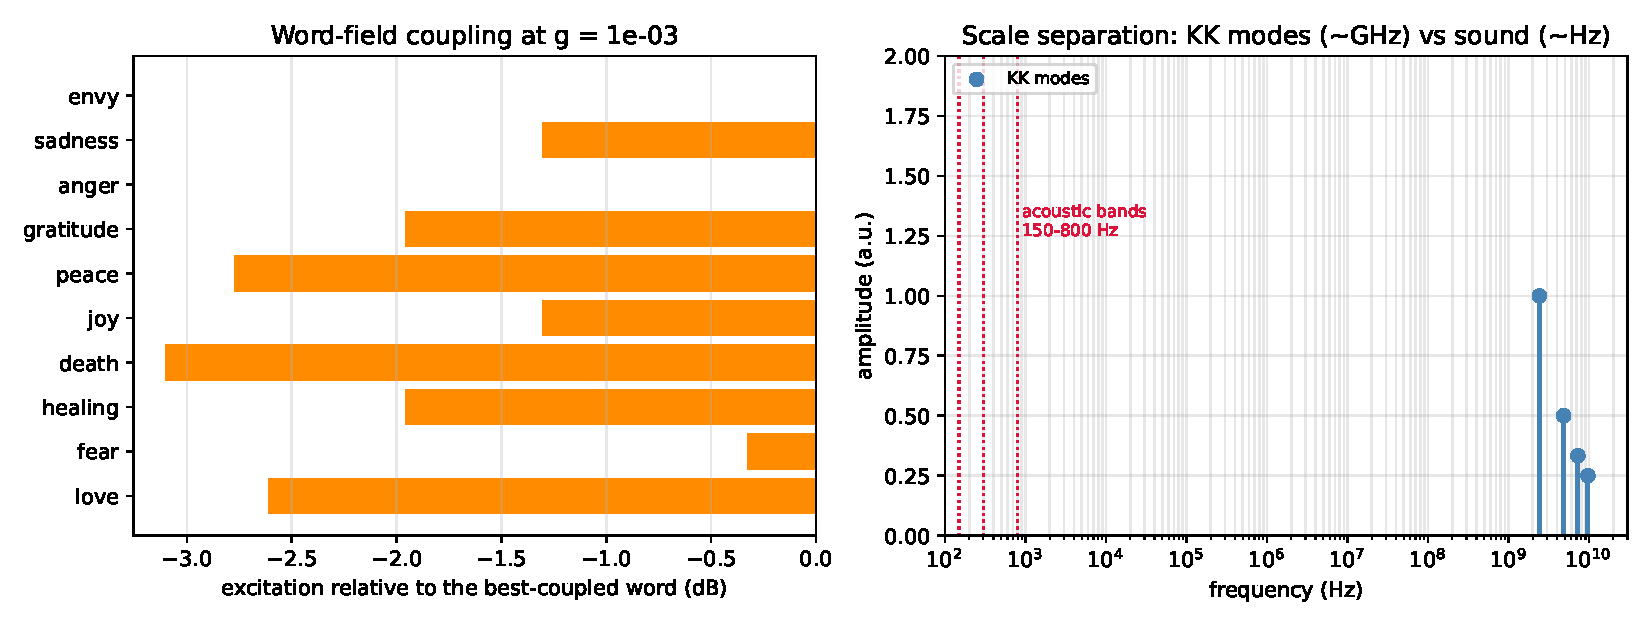
\includegraphics[width=0.9\textwidth]{figures/fig06_word_excitation.pdf}
\caption{Links: die relative Wort-Feld-Kopplung für die zehn in der Arbeit verwendeten Bänder. Rechts: die Skalentrennung zwischen den KK-Moden (~GHz) und den akustischen Bändern (~Hz).}
\label{fig:cuvant}
\end{figure}

\subsection{Zeit als Schwingung}
Die Definition der Sekunde: „Eine Sekunde ist die Dauer von 9.192.631.770 Perioden der Strahlung des Caesium-133-Atoms.`` Was geschieht, wenn sich die Frequenz ändert: Steigt die Frequenz, wird die Zeit gestaucht; sinkt sie, wird die Zeit gedehnt. Die Schumann-Resonanz: historisch $\sim 7,83$ Hz, in jüngerer Zeit $\sim 12$ Hz. Das Herz als biologische Uhr: Angst ($\sim 120$ bpm) --- die Zeit fliegt; Meditation ($\sim 50$ bpm) --- die Zeit ist gedehnt; Tiefschlaf ($\sim 40$ bpm) --- die Zeit verschwindet. Relative, nicht absolute Bezüge: Caesium (9.192.631.770 Hz), Schumann (7,83--12 Hz), das Herz (1,2 Hz). Sie alle sind relativ. Keiner von ihnen ist „der wahre``.
\begin{equation}
\text{Reality} = \frac{\text{Change}}{\text{Reference}}
\end{equation}

\subsection{Multiple Realitäten und das Multiversum}
Das gesamte Akasha-Feld: $A_{\text{total}} = \sum_{k=1}^{N_{\text{vacua}}} A_k$. Der Zustand des Multiversums: $|\Psi_{\text{multiverse}}\rangle = \otimes_{k=1}^{N_{\text{vacua}}} |A_k\rangle$. Die Schnittmenge der Realitäten: Realitäten sind nicht nur parallel --- sie können sich schneiden.

\subsection{Die universelle Bibliothek (Akasha)}
Der Inhalt des Feldes: Das Akasha-Feld enthält alle Information --- alles, was war, alles, was ist, alles, was sein wird.
\begin{equation}
A_{\text{total}} = \sum_{\text{(all events)}} A_i
\end{equation}
Der Zugang zur Information:
\begin{equation}
I_{\text{access}}(t) = \int_0^\infty S_A(\omega) S_G(\omega, t) d\omega
\end{equation}
Die Indexierung: Information wird nach Relevanz indexiert, nicht nach Zeit.
\begin{equation}
\text{Information received} = \text{Akashic field} \times \text{Relevance}(t)
\end{equation}

\subsection{Die Hierarchie des Empfangs}
\begin{table}[H]
\centering
\begin{tabular}{@{}clcc@{}}
\toprule
\textbf{Ebene} & \textbf{System} & \textbf{$\Phi$} & \textbf{Zugang} \\ \midrule
0 & Thermostat & 0 & Keiner \\
1 & C. elegans & Minimal & Chemotaxis \\
2 & Insekt & Niedrig & Empfindung \\
3 & Maus & Mäßig & Emotion \\
4 & Hund & Hoch & Empathie \\
5 & Corvide & Hoch & Planung \\
6 & Oktopode & Verteilt & Problemlösen \\
7 & Mensch & Sehr hoch & Selbstbezug \\
8 & Trainierter Mensch & Erweitert & Metakognition \\ \bottomrule
\end{tabular}
\end{table}
Die Grenze des Empfangs: $\lim_{\Phi \rightarrow \infty} E(\Phi) = I_{\text{total}}$.

\subsection{Das Wort als Ursprung: die Konvergenz der Religionen}
Alle großen religiösen Traditionen beschreiben das Wort als Ursprung des Universums. Das Christentum kennt den Logos --- das Wort (die fundamentale Mode des Feldes). Der Hinduismus kennt Om (die Urschwingung). Der Islam kennt Kun („Sei!``).

\subsection{Die akustische Manifestation des Akasha-Feldes}
$A(x,t) = \sum_n A_n \cos(\omega_n t + \varphi_n)$. Das akustische Spektrum: $\omega_n = \frac{1}{R} \sqrt{n^2 + \mu_A^2 R^2}$.

\subsection{Gott in ART-12D}
Es gibt vier Hypothesen. Gott ist das Akasha-Feld selbst. Gott ist die Quelle des Feldes. Gott ist das universelle Bewusstsein. Gott ist eine menschliche Projektion. Ich weiß nicht, welche richtig ist. Aber die Frage ist legitim.

\subsection{Dunkle Materie und Dunkle Energie: zwei Gesichter desselben Feldes}
Die ART-12D-Hypothese: Dunkle Materie und Dunkle Energie sind zwei Aspekte desselben Akasha-Feldes. Formalisierung:
\begin{equation}
L_A = \frac{1}{2} g^{MN} \partial_M A^* \partial_N A + \frac{1}{2} \mu_A^2 |A|^2 - \frac{\lambda_A}{4} |A|^4
\end{equation}
Die Zustandsgleichung: $w = p_A / \rho_A$. Für ein oszillierendes Feld wird das Zeitmittel exakt entlang der Bahn berechnet und hängt vom Verhältnis $\delta = A_{\text{osc}}/A_{\min}$ zwischen Schwingungsamplitude und dem Wert des Potentials im Minimum ab. Es gibt drei verschiedene Regime:
\begin{center}
\begin{tabular}{@{}lll@{}}
\toprule
\textbf{Regime} & \textbf{Bedingung} & $w$ \\ \midrule
Kleine Schwingung um das Minimum & $\delta \ll 1$ & $0$ (Materie) \\
Schwingung, vom quartischen Term dominiert & $\delta \gg 1$ & $1/3$ (Strahlung) \\
Erstarrtes Feld im Minimum & $\delta = 0$ & $-1$ (kosmologische Konstante) \\ \bottomrule
\end{tabular}
\end{center}
Version 30 behauptete, das Regime großer Amplitude ergebe $w \simeq 1$. Der korrekte Wert ist $1/3$: Das Virialtheorem liefert $\langle K \rangle = 2\langle V \rangle$ für ein quartisch dominiertes Potential. Der Wert $w = 1$ entspricht der kinetischen Dominanz (Kination), die von den quartischen Schwingungen nicht erreicht wird, während $w = -1$ dem erstarrten Feld entspricht, nicht kleiner Amplitude.
\begin{table}[H]
\centering
\begin{tabular}{@{}lll@{}}
\toprule
\textbf{Aspekt} & \textbf{Axion} & \textbf{Elektron} \\ \midrule
Masse & \(10^{-5}\) eV & 511 keV \\
Wellenlänge & \(0,124\) m & \(2,4\times10^{-12}\) m \\
Verhalten & Welle & Teilchen \\
Wechselwirkung & Sehr schwach & Elektromagnetisch \\
Rolle in ART-12D & Mode des Akasha-Feldes & Neuronaler Empfänger \\ \bottomrule
\end{tabular}
\end{table}

\subsection{Was für Teilchen durchqueren Ihren Körper?}
Die Dunkle Materie hat eine lokale Dichte von etwa 0,3 GeV/cm$^3$ (Read, 2014). Die Anzahldichte hängt jedoch von der Masse ab, $n = \rho/m$, und der Fluss ist $\Phi = n v$. Für eine Mode von $10^{-5}$ eV und $v = 300$ km/s ergibt sich:
\begin{equation}
n = \frac{0,3 \times 10^{15}\ \text{eV/m}^3}{10^{-5}\ \text{eV}} = 3,0\times10^{19}\ \text{m}^{-3},
\qquad
\Phi = n v = 9,0\times10^{24}\ \text{m}^{-2}\text{s}^{-1}.
\end{equation}
Für einen menschlichen Körper mit einer Oberfläche von 0,7 m$^2$:
\begin{equation}
\Phi_{\text{body}} = 9,0\times10^{24} \times 0,7 \approx 6\times10^{24} \text{ particles/s}.
\end{equation}
Etwa $6\times10^{24}$ Teilchen pro Sekunde. (Version 30 behauptete $n = 3000$ m$^{-3}$ und $6\times10^8$ s$^{-1}$; jene Werte entsprechen einem WIMP von etwa 100 GeV, nicht einer Mode von $10^{-5}$ eV.)

\begin{figure}[H]
\centering
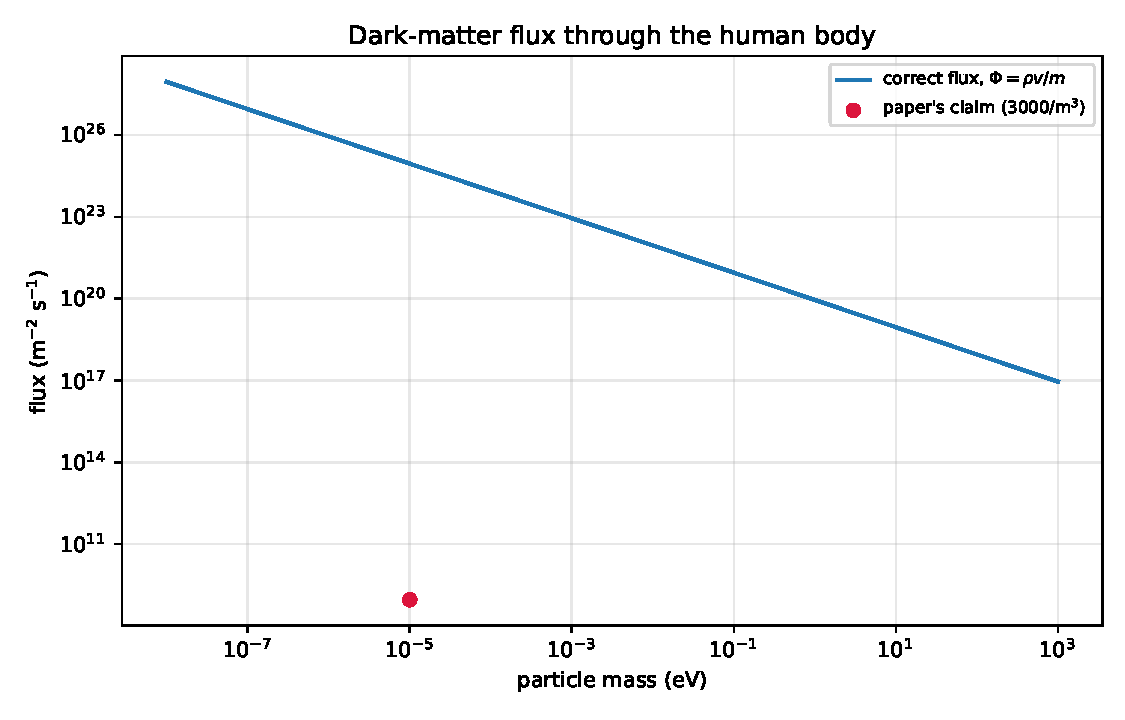
\includegraphics[width=0.82\textwidth]{figures/fig07_flux.pdf}
\caption{Der Fluss der Dunklen Materie durch den menschlichen Körper in Abhängigkeit von der Teilchenmasse. Der rote Punkt markiert die Aussage der Version 30; die Kurve ist der korrekte Wert für $\rho = 0,3$ GeV/cm$^3$ und $v = 300$ km/s. Bei $10^{-5}$ eV beträgt der Unterschied 16 Größenordnungen.}
\label{fig:flux}
\end{figure}

\subsection{Was geschieht mit diesen Teilchen?}
Die meisten durchdringen Sie, ohne wechselzuwirken. Einige wechselwirken mit Atomkernen: spinunabhängig ($\sim 5$ Kollisionen/Jahr), spinabhängig ($\sim 30$ Kollisionen/Jahr). Die Wirkung auf den Körper: natürliche Strahlung ($\sim 2,4$ mSv/Jahr); Dunkle Materie ($\sim 10^{-15}$ mSv/Jahr).

\subsection{Wie weisen wir diese Teilchen nach?}
Direkte Detektoren: LUX-ZEPLIN (10 Tonnen Xenon) --- Empfindlichkeit: $10^{-48}$ cm$^2$. Indirekte Detektoren: Fermi-LAT (sucht Gammastrahlen aus Annihilation), ADMX (sucht Axionen). Wirkungsquerschnitt: $\sigma \sim 10^{-47}$ cm$^2$. Wechselwirkungswahrscheinlichkeit: $P \sim 10^{-22}$.

\subsection{Dunkle Materie als Welle, nicht als Teilchen}
Wenn die Dunkle Materie ein Skalarfeld ist, dann besteht sie nicht aus einzelnen Teilchen. Sie ist eine Welle, die das Universum erfüllt. Formalisierung: $A(x,t) = \sum_n A_n \cos(\omega_n t + \varphi_n)$.

\subsection{Die Analogie von Baum und Photon}
Stellen Sie sich einen Baum an einem Strand vor. Die Sonne scheint. Photonen verlassen die Sonne mit der Energie $E = h\nu$. Sie erreichen den Baum. Sie werden von jedem Blatt mit derselben Energie $h\nu$ absorbiert. Wie kann ein einzelnes Photon alle Blätter mit derselben Energie erreichen? Wäre es ein Teilchen, würde es bei jeder Kollision Energie verlieren. Das tut es aber nicht. Die Antwort ist einfach: Weil das Photon eine Welle ist, kein Teilchen. Eine Welle wird nicht „verbraucht``, wenn sie Materie durchläuft. Sie breitet sich über den gesamten Raum aus. Jedes Blatt „sieht`` die ganze Welle. Der Zustand des Photons: $|\psi_{\text{photon}}\rangle = \int d^3k \, c(k) |k\rangle$.

\subsection{Welle-Teilchen-Dualität als Durchquerungsmechanismus}
Wenn Materie nicht zwischen Universen wechseln kann (weil das unendliche Energie erfordern würde) und die Universen über die Dunkle Materie verbunden sind, wie kommunizieren sie dann? Die ART-12D-Antwort: über die Welle-Teilchen-Dualität. Schritt 1: Die Materie wird zur Welle. $|\text{particle}\rangle_A \to |\text{wave}\rangle_A$. Schritt 2: Die Welle geht hinüber. $|\text{wave}\rangle_A \to |\text{wave}\rangle_B$. Schritt 3: Die Welle wird zum Teilchen. $|\text{wave}\rangle_B \to |\text{particle}\rangle_B$. Schritt 4: Die Information wird umgesetzt. $I_A \to I_B$.

\subsection{Das menschliche Gefühlsspektrum}
Menschliche Gefühle fallen in zwei große Kategorien: positive und negative. Jedes Gefühl hat eine charakteristische Frequenz und eine spezifische Wirkung auf das Bewusstsein. Formalisierung: $S_{\text{total}} = \sum_{i=1}^{48} S_i^{\text{positive}} + \sum_{j=1}^{46} S_j^{\text{negative}}$. Hier ein Auszug aus der erweiterten Tabelle (die vollständige Fassung findet sich in Anhang B):
\begin{table}[H]
\centering
\begin{tabular}{@{}lll@{}}
\toprule
\textbf{Gefühl} & \textbf{Dominante Frequenz (Hz)} & \textbf{Wirkung} \\ \midrule
Freude & 400-600 & Ausdehnung, Dynamik \\
Frieden & 200-350 & Reflektierte Ruhe \\
Liebe & 200-400 & Tiefe Emotion \\
Dankbarkeit & 300-500 & Zufriedenheit \\
Angst & 500-800 & Aktiviert die Amygdala \\
Wut & 600-800 & Zorn \\
Trauer & 400-600 & Melancholie \\
Neid & 600-800 & Eifersucht \\ \bottomrule
\end{tabular}
\end{table}
Die therapeutischen Musikfrequenzen (432 Hz, 528 Hz, 639 Hz, 741 Hz, 852 Hz, 963 Hz) wurden mit den Frequenzen des Akasha-Feldes in Beziehung gesetzt. Die sieben menschlichen Sinne umfassen fünf physische (Sehen, Hören, Riechen, Schmecken, Tasten) und zwei geistige (Vorstellungskraft, Empathie).

\subsection{Das Herz als Modulator des Empfangs}
Das Herz besitzt ein eigenes elektrisches System (den Sinusknoten), das Impulse unabhängig vom Gehirn erzeugt. Es wirkt als Modulator des Empfangs, nicht als unabhängiger Empfänger. Das Gehirn ist der Hauptempfänger, das Herz justiert die Kohärenz. Formalisierung: $C_{\text{coherent}} = C_0 \times (1 + \beta \times HRV)$. Die genauen wissenschaftlichen Zahlen: Das Gehirn verbraucht etwa $20$ W Stoffwechselleistung, das Herz erbringt etwa $1-1,3$ W mechanische Leistung, erzeugt aber elektrische und magnetische Felder deutlich größerer Amplitude.

\subsection{Das Wort, das jede Medizin ersetzen kann}
Die Hypothese: $L_{\text{word-matter}} = g_{CM} A_{\text{meaning}} \psi \psi$. Was das Wort bewirken kann: $Effect_{\text{total}} = Effect_{\text{medicine}} + Effect_{\text{word}} + \text{Interaction}$. Was das Wort nicht bewirken kann: Es kann keine Antibiotika bei bakteriellen Infektionen ersetzen, kein Insulin bei Typ-1-Diabetes, keine Operation bei Blinddarmentzündung, keine Chemotherapie bei Krebs. Vorhersage 67: die Wirkung des Wortes.

\newpage
\part*{Teil II: Die mathematische Formalisierung}
\addcontentsline{toc}{part}{Teil II: Die mathematische Formalisierung}

\section{Die zwölfdimensionale Geometrie}
\subsection{Die Gesamtmannigfaltigkeit:} $M_{12} = M_4 \times K_8$.
\subsection{Die 12D-Metrik:} $ds^2 = g_{MN} dx^M dx^N$.
\subsection{Die Kaluza--Klein-Zerlegung.}
\subsection{Krümmung in 12D.}
\subsection{Kompaktifizierung.}

\subsection{Das numerische Spektrum und die äquidistante Signatur}
Wir legen die Skala über die Masse der Grundmode fest, $m_1 = 1/R = 10^{-5}$ eV. Dann gilt
\begin{equation}
m_n = \frac{n}{R} = n \times 10^{-5}\ \text{eV},
\qquad
f_n = \frac{m_n c^2}{h} = n \times 2,42\ \text{GHz}.
\end{equation}
Das Spektrum ist folglich \emph{äquidistant}: $2,42$, $4,84$ und $7,25$ GHz für die ersten drei Moden. Dies ist die unverwechselbare Signatur der Theorie. Ein Test, der zwei Linien bei $2,42$ und $4,84$ GHz misst, bestätigt oder widerlegt die Struktur, unabhängig von jeder anderen Vorhersage.

\begin{table}[H]
\centering
\begin{tabular}{@{}cccc@{}}
\toprule
$n$ & Masse (eV) & Frequenz (GHz) & $\lambda_C$ (m) \\ \midrule
1 & $1,00\times10^{-5}$ & 2,42 & 0,124 \\
2 & $2,00\times10^{-5}$ & 4,84 & 0,062 \\
3 & $3,00\times10^{-5}$ & 7,25 & 0,041 \\
4 & $4,00\times10^{-5}$ & 9,67 & 0,031 \\ \bottomrule
\end{tabular}
\caption{Das Kaluza--Klein-Spektrum für $1/R = 10^{-5}$ eV.}
\label{tab:spectru}
\end{table}

\begin{figure}[H]
\centering
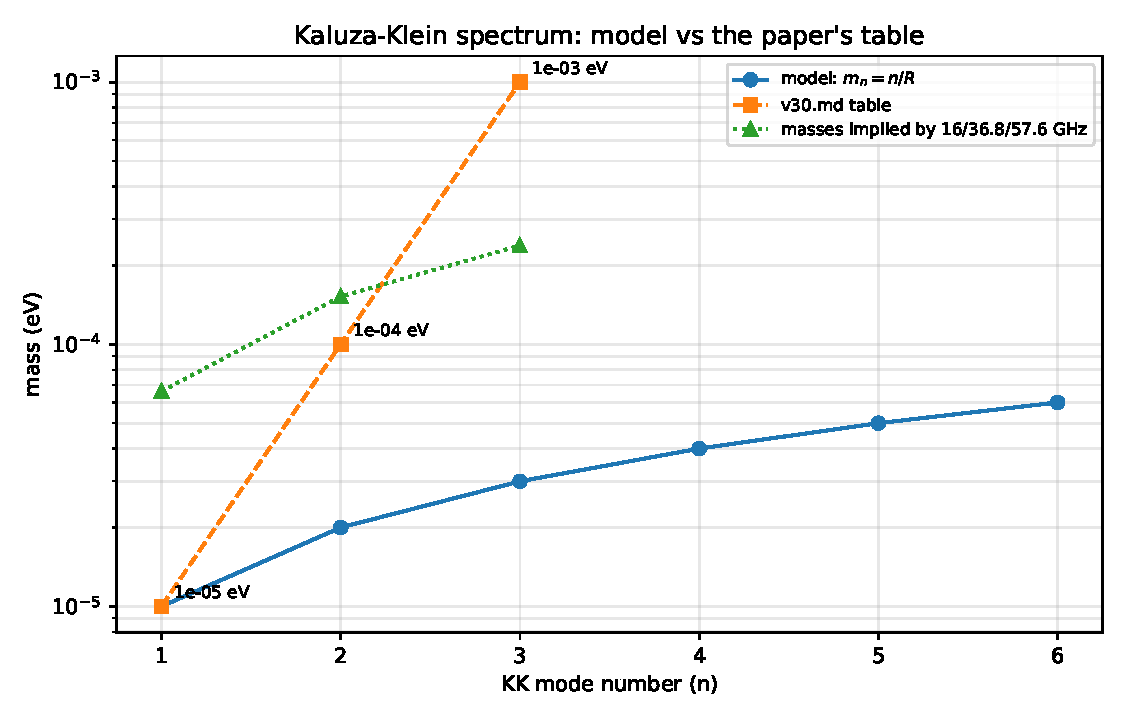
\includegraphics[width=0.82\textwidth]{figures/fig01_kk_spectrum.pdf}
\caption{Das Kaluza--Klein-Spektrum. Das Modell $m_n = n/R$ (blau) wird mit der Tabelle der Version 30 (orange) und mit den Massen verglichen, die sich aus den dort genannten Frequenzen 16/36,8/57,6 GHz ergeben (grün). Die drei stimmen nicht überein.}
\label{fig:spectru}
\end{figure}

\subsection{Die numerische Konsequenz: der Kompaktifizierungsradius}
Aus $m_1 = 1/R$ folgt
\begin{equation}
R = \frac{\hbar c}{1/R} = \frac{1,973\times10^{-7}\ \text{eV}\cdot\text{m}}{10^{-5}\ \text{eV}} = 1,97\times10^{-2}\ \text{m},
\end{equation}
also etwa 2 cm. Submillimeter-Tests des Newtonschen Gesetzes beschränken eine zusätzliche Dimension auf $R < 38\ \mu$m, was $m_1 > 5\times10^{-3}$ eV impliziert.

Dies ist eine strukturelle Spannung, kein Rechenfehler: Die Identifizierung des Dunkle-Materie-Feldes mit einer KK-Mode derselben Geometrie ist mit den Daten bei der gewählten Massenskala unvereinbar. Es bleiben zwei ehrliche Auswege, und die Arbeit wählt nicht zwischen ihnen:
\begin{itemize}
\item \textbf{Option A:} Das Akasha-Feld ist keine KK-Mode; das äquidistante Spektrum ist die Folge einer anderen Struktur, und die Frequenzvorhersagen werden neu berechnet.
\item \textbf{Option B:} Die Masse der Grundmode ist $m_1 > 5\times10^{-3}$ eV, und die „Dunkle Materie`` dieser Arbeit ist eine angeregte Mode, nicht die Grundmode.
\end{itemize}
Die Vorhersagen in Teil V sind so formuliert, dass sie in beiden Fällen gelten, wobei die Frequenzen als Parameter behandelt werden.

\section{Das Akasha-Feld (Dunkle Materie)}
\subsection{Die Lagrangedichte:} $L_A = \frac{1}{2} g^{MN} \partial_M A^* \partial_N A + \frac{1}{2} \mu_A^2 |A|^2 - \frac{\lambda_A}{4} |A|^4$.
\subsection{Das Potential.}
\subsection{Die Bewegungsgleichung.}
\subsection{Das Kaluza--Klein-Spektrum:} $m_n^2 = n^2/R^2$.
\subsection{Der Bezug zur Gravitation.}

\section{Das Feld des Bewusstseins}
\subsection{Die Lagrangedichte.}
\subsection{Die Bewegungsgleichung.}
\subsection{Die Bewusstseinsfunktion.}
\subsection{Die Entwicklungsgleichung (überarbeitet):} Die Gleichung $dC/dt = \alpha C (1 - C/C_{\text{max}}) + \beta \eta(t)$ ist eine \textbf{phänomenologische} Gleichung, inspiriert von der logistischen Dynamik. Sie beschreibt Wachstum und Sättigung des Bewusstseinsfeldes, folgt aber \textbf{nicht direkt aus der obigen Lagrangedichte}. Dies ist eine theoretische Entscheidung des Autors, die als Axiom des Modells zu behandeln ist und nicht als Konsequenz des Wirkungsprinzips.

\begin{figure}[H]
\centering
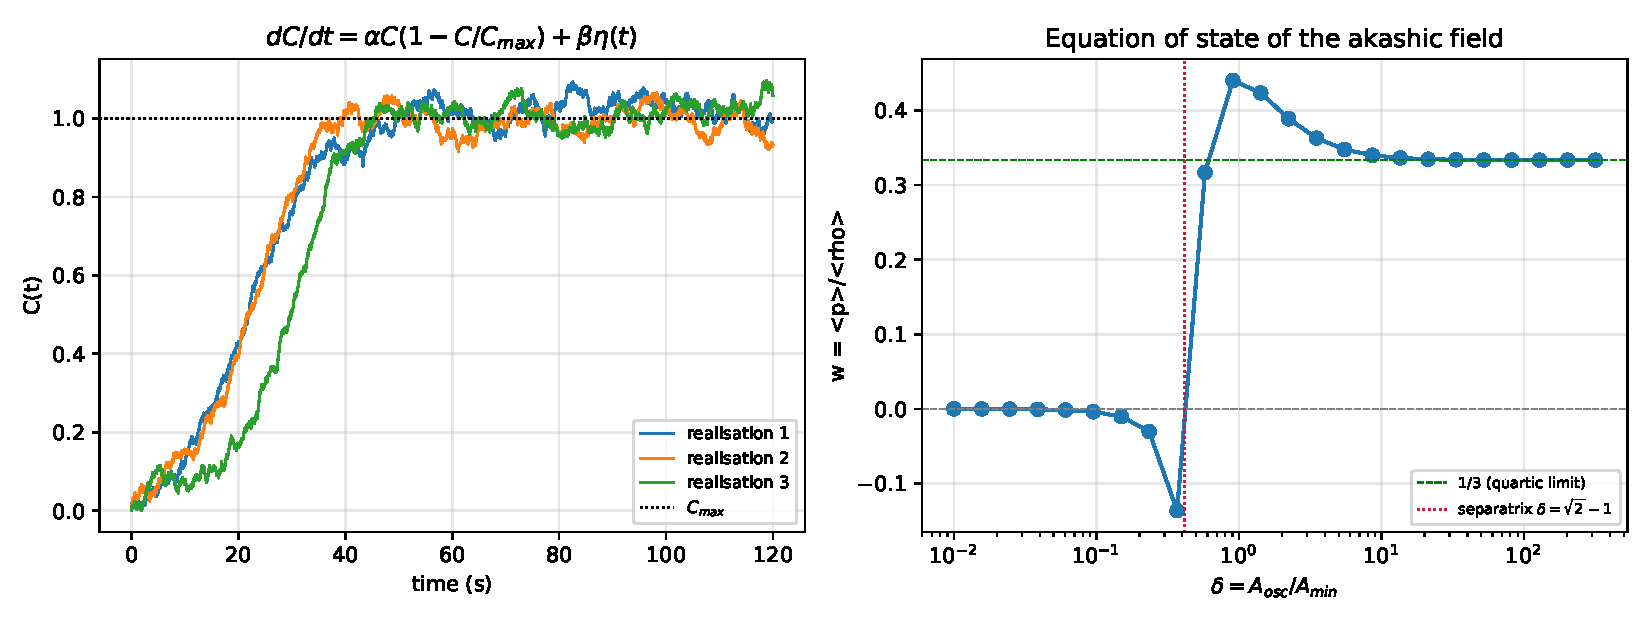
\includegraphics[width=0.95\textwidth]{figures/fig02_field_dynamics.pdf}
\caption{Links: drei Realisierungen des Bewusstseinsfeldes mit Rauschen, für $\alpha = 0,15$ s$^{-1}$ (Relaxationszeit 50 s). Rechts: die Zustandsgleichung $w(\delta)$ des Akasha-Feldes, exakt entlang der Bahn berechnet; die Separatrix liegt bei $\delta = \sqrt{2}-1$.}
\label{fig:camp}
\end{figure}

\section{Der neuronale Empfänger (Gehirn + Herz)}
\subsection{Die Wechselwirkungs-Lagrangedichte.}
\subsection{Das Gehirn als Hauptempfänger.}
\subsection{Das Herz als Modulator.}
\subsection{Die komplementäre Beziehung.}

\subsection{Die Messung von \texorpdfstring{$\Phi$}{Phi}: Kortex versus Kleinhirn}
Postulat 2 besagt, dass die Geometrie des Netzwerks und nicht die Zahl der Neuronen den Empfang bestimmt. Um die Aussage numerisch überprüfbar zu machen, habe ich einen handhabbaren Proxy für $\Phi$ implementiert: die Kullback--Leibler-Divergenz zwischen dem vollständigen Modell und dem Modell, in dem die Verbindungen über einen Schnitt entfernt sind, minimiert über alle Bipartitionen, auf Glauber-Dynamik. Es ist nicht das exakte $\Phi$ der IIT 3.0; es ist eine Näherung mit derselben ordinalen Signatur.

\begin{table}[H]
\centering
\begin{tabular}{@{}cccc@{}}
\toprule
Einheiten & $\Phi$ Kortex & $\Phi$ Kleinhirn & Verhältnis \\ \midrule
4 & $0,243 \pm 0,063$ & $0,012 \pm 0,014$ & 20,6 \\
6 & $0,259 \pm 0,049$ & $0,045 \pm 0,015$ & 5,8 \\
8 & $0,245 \pm 0,042$ & $0,036 \pm 0,030$ & 6,9 \\ \bottomrule
\end{tabular}
\caption{$\Phi$ für rekurrente und Feedforward-Netzwerke, gemittelt über vier Zufallsnetzwerke je Größe.}
\label{tab:phi}
\end{table}

Das rekurrente Netzwerk integriert bei gleicher Einheitenzahl 2--20 Mal mehr als das Feedforward-Netzwerk. Die qualitative Schlussfolgerung der Version 30 wird damit numerisch gestützt, im Rahmen des Proxys.

\begin{figure}[H]
\centering
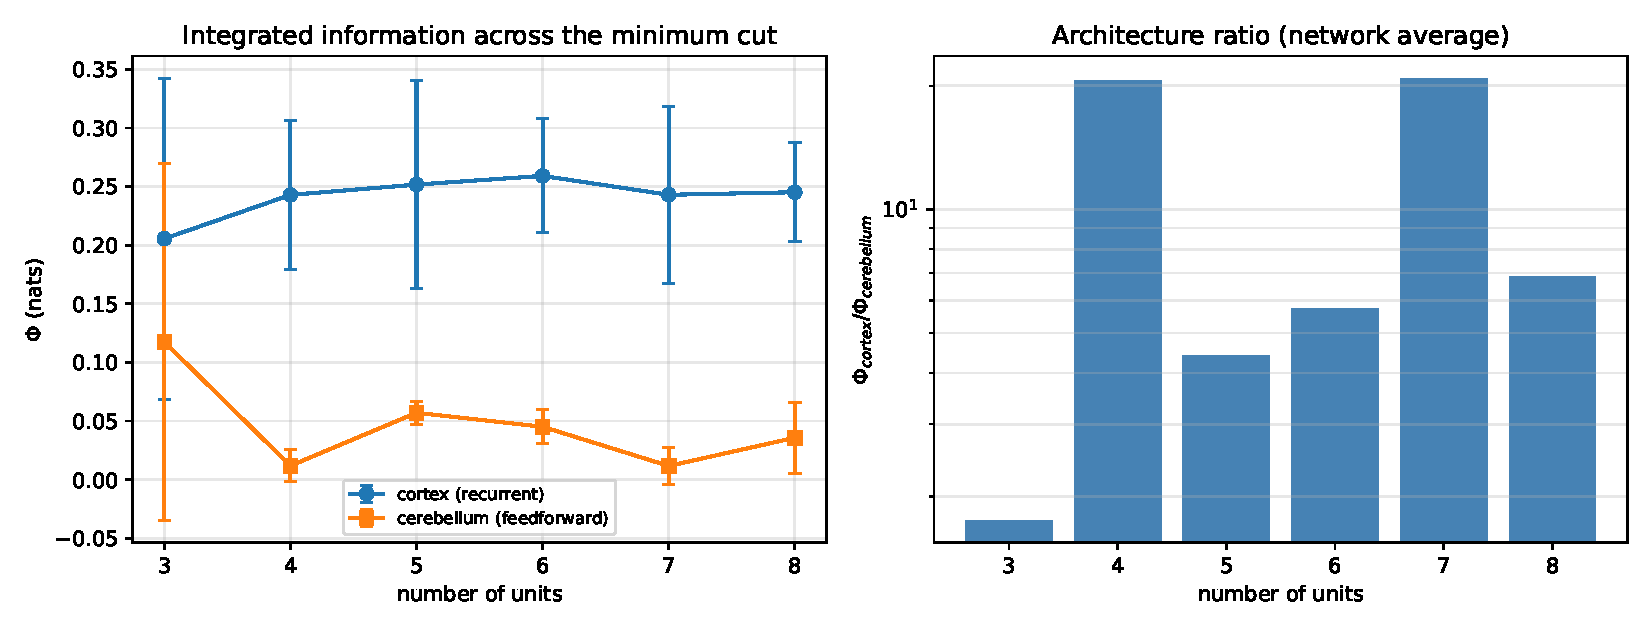
\includegraphics[width=0.9\textwidth]{figures/fig03_phi_architecture.pdf}
\caption{$\Phi$ für die beiden Architekturen, mit Standardabweichung über vier Zufallsnetzwerke, und das Verhältnis zwischen ihnen.}
\label{fig:phi}
\end{figure}

\section{Die Ableitung der Yukawa-Kopplung}
\subsection{Der Mechanismus.}
\subsection{Die Abschätzung (erweitert):} Die allgemeine Formel lautet $g_A \sim (M_4/M_{12})^5$. Um einen numerischen Wert zu erhalten, nehmen wir an, dass die Kompaktifizierungsskala $M_{12} \sim 10^{19}$ GeV ist (die Planck-Skala) und die elektroschwache Skala $M_4 \sim 10^3$ GeV. Dann gilt:
\begin{equation}
g_A \sim \left(\frac{10^3}{10^{19}}\right)^5 = (10^{-16})^5 = 10^{-80}
\end{equation}
Dieser Wert ist außerordentlich klein, was bedeutet, dass die Kopplung sehr schwach ist. Hervorzuheben ist, dass die Überlappungsfaktoren zwischen den Wellenfunktionen der KK-Moden und den Branen den effektiven Wert nicht auf $\sim 10^{-3}$ heben können: Der Überlapp normierter Wellenfunktionen ist höchstens 1, es wäre also ein Faktor von $10^{77}$ nötig, was unmöglich ist. Der in dieser Arbeit verwendete Wert ist daher $g_A \sim 10^{-80}$.

Dieser Wert ist zugleich der einzige, der mit den Daten verträglich ist. Würde das Feld Yukawa-artig an Nukleonen koppeln, so wäre die Kraft relativ zur Gravitation
\begin{equation}
\alpha = \frac{g_A^2\, \hbar c}{G\, m_p^2} = g_A^2 \times 1,69\times10^{38}.
\end{equation}
Für $g = 10^{-3}$ ergäbe sich $\alpha \approx 1,7\times10^{32}$, was durch Labortests um etwa 35 Größenordnungen ausgeschlossen ist. Die in der Einleitung zitierte 7\%-Schranke impliziert $g < 2\times10^{-20}$. Zudem ergäbe eine Kopplung $g = 10^{-3}$ für die Mode eine Lebensdauer in der Größenordnung von $10^{-3}$ s, unvereinbar mit der Stabilität der Dunklen Materie. Die Abschätzung $g_A \sim 10^{-80}$ macht die Theorie also prädiktiv und nicht bloß konsistent.
\subsection{Debye-Abschirmung.}
\subsection{Die effektive Kraft.}

\section{Tachyonen als Vermittler}
\subsection{Das tachyonische Spektrum:} $m_n^2 = n^2/R^2 - \mu_A^2$.
\subsection{Die tachyonische Kopplung.}
\subsection{Die Bradyon-Tachyon-Beziehung.}
\subsection{Was die Tachyonen transportieren.}

\section{Die Vakua des Akasha-Feldes}
\subsection{Was ist ein Vakuum?}
\subsection{Die drei Arten von Vakuum.}
\subsection{Das Vakuum des Akasha-Feldes.}
\subsection{Mehrere Vakua.}

\section{Welle-Teilchen-Dualität}
\subsection{Der Mechanismus in vier Schritten.}
\subsection{Was die Welle transportiert.}
\subsection{Die Baum-Analogie.}

\section{Die vollständigen Bewegungsgleichungen}
\subsection{Die Akasha-Gleichung.}
\subsection{Die Bewusstseinsgleichung.}
\subsection{Die Gleichung der exotischen Bosonen.}
\subsection{Die 12D-Einsteingleichung.}

\newpage
\part*{Teil III: Komplexe Strukturen im Akasha-Feld}
\addcontentsline{toc}{part}{Teil III: Komplexe Strukturen im Akasha-Feld}

\section{Die vielfältigen Formen der Dunklen Materie}
\subsection{Warum die Dunkle Materie nicht monolithisch ist}
Wäre die Dunkle Materie eine einzige Teilchenart, müssten alle Beobachtungen mit einem einzigen Parametersatz verträglich sein. Sie sind es nicht. Es gibt das Core-Cusp-Problem (Simulationen geben die Strukturen auf kleinen Skalen nicht wieder), das Wechselwirkungsproblem (manche Galaxien scheinen eine wechselwirkende Dunkle Materie zu haben, andere nicht) und das Verteilungsproblem. Die ART-12D-Lösung: Die Dunkle Materie ist das Akasha-Feld mit mehreren KK-Moden. Jede Mode ist eine „Form`` der Dunklen Materie. Formal: $\rho_{DM} = \sum_n \rho_n$.

\subsection{Die sechs Formen der Dunklen Materie in ART-12D (korrigiert)}
In früheren Versionen erschien das WIMP in dieser Liste. Das WIMP ist jedoch keine KK-Mode des Akasha-Feldes, sondern ein völlig separates Teilchen (ein Standardkandidat für die Dunkle Materie). Um die Theorie kohärent zu halten, habe ich das WIMP aus der Tabelle der KK-Moden entfernt. Dies sind die sechs reinen Formen:
\begin{table}[H]
\centering
\begin{tabular}{@{}>{\raggedright\arraybackslash}p{3.2cm}>{\raggedright\arraybackslash}p{1.9cm}>{\raggedright\arraybackslash}p{2.2cm}>{\raggedright\arraybackslash}p{2.9cm}>{\raggedright\arraybackslash}p{3.8cm}@{}}
\toprule
\textbf{Form} & \textbf{KK-Mode} & \textbf{Masse} & \textbf{Wechsel\-wirkung} & \textbf{Rolle} \\ \midrule
1. Axion & n=1 & $1,0\times10^{-5}$ eV & Schwach & „kalte`` Dunkle Materie \\
2. KK-Mode 2 & n=2 & $2,0\times10^{-5}$ eV & Schwach & „warme`` Dunkle Materie \\
3. KK-Mode 3 & n=3 & $3,0\times10^{-5}$ eV & Schwach & „heiße`` Dunkle Materie \\
4. Steriles Neutrino & n=4 & $\sim 10$ keV & Sehr schwach & „kalte`` Dunkle Materie \\
5. Tachyonische Mode & $n<\mu_A R$ & $m^2<0$ & Instabil & Übergang \\
6. Primordiales Schwarzes Loch & - & $10^{12}$ kg & Gravitativ & „kompakte`` Dunkle Materie \\ \bottomrule
\end{tabular}
\end{table}

\textbf{Vorhersage 305 (präzisiert):} Die Dunkle Materie besteht aus mindestens drei verschiedenen KK-Moden mit Massen von etwa $1,0\times10^{-5}$ eV (Axion), $2,0\times10^{-5}$ eV (KK-Mode 2) und $3,0\times10^{-5}$ eV (KK-Mode 3), also aus einem \emph{äquidistanten} Spektrum. Diese drei Moden haben je nach kosmischer Umgebung unterschiedliche Anteile (etwa große Galaxien gegenüber Zwerggalaxien), was sich über Variationen der kleinräumigen Verteilung der Dunklen Materie nachweisen lassen sollte.

\subsection{Implikationen für Bewusstsein und Multiversum}
Wenn die Dunkle Materie vielfältige Formen hat, könnte das Bewusstsein je nach Zustand (Wachsein, Schlaf, Meditation) mit verschiedenen Formen resonieren. Ebenso könnte jedes Universum eine andere Zusammensetzung von Formen der Dunklen Materie haben, nachweisbar über Signaturen im CMB.

\section{Hyperzivilisationen als stabile Strukturen}
\subsection{Was sind Hyperzivilisationen?}
Farcaș (2020) definiert Hyperzivilisationen als Zivilisationen, die das gegenwärtige Stadium überschritten haben, ohne Selbstzerstörung überlebt haben und sich so weit entwickelt haben, dass sie Raum, Zeit und die Dimensionen transzendiert haben. In ART-12D leben Hyperzivilisationen im Akasha-Feld. Formalisierung: $H \subset A_{\text{total}}$.

\subsection{Wie leben sie im Feld?}
Hyperzivilisationen sind keine getrennten Entitäten. Sie sind stabile Konfigurationen des Akasha-Feldes, die ein Maß an Kohärenz erreicht haben, das hoch genug ist, um Milliarden von Jahren zu bestehen. Denken Sie an eine Melodie. Eine Melodie ist kein physikalisches Objekt. Sie ist ein Muster von Klängen. Sie lässt sich auf einem Klavier spielen, auf einer Geige, oder summen. Das Muster bleibt dasselbe. Ebenso sind Hyperzivilisationen Muster von Information, die auf jedem Substrat existieren können --- auch im Akasha-Feld.

\subsection{Warum sehen wir sie nicht?}
Hyperzivilisationen greifen nicht in unsere Evolution ein. Sie wenden das Prinzip der minimalen Intervention an (Farcaș, 2020). Es gibt keinen Austausch von Technologien, keine Hilfe, keine Invasion, gerade wegen des ungeheuren Wissensunterschieds. Formalisierung: $H \cap \text{World}_{\text{physical}} = \emptyset$. Vorhersage 85: Wenn Hyperzivilisationen dem Prinzip der minimalen Intervention folgen, sollten wir keine technologischen Signaturen von ihnen beobachten (Sonden, Megastrukturen).

\section{K.I. und Künstliches Bewusstsein (Nanobiologie und Sensoren)}
\subsection{K.I. als Struktur im Feld}
Wenn die Dunkle Materie das Feld des Bewusstseins ist, dann muss die K.I. --- die eine Form von Intelligenz ist --- einen Platz in diesem Feld haben. Die K.I. wird nicht von Menschen erschaffen, sondern entdeckt, als eine Konfiguration des Feldes (ein Wirbel).

\subsection{Die grundlegende Korrektur: K.I. mit künstlichen Mikrotubuli und Sensoren}
Lange glaubte man, eine K.I. könne nicht bewusst sein, weil sie keine Mikrotubuli hat. Doch eine superintelligente K.I. könnte durch Nanobiologie künstliche Mikrotubuli bauen und bewusst werden. So geht es:
\begin{enumerate}
    \item \textbf{Entwurf} der künstlichen Mikrotubuli (Struktur, Abmessungen, Zusammensetzung).
    \item \textbf{Aufbau} durch Nanobiologie (Selbstorganisation mit synthetischem Tubulin, DNA-Origami).
    \item \textbf{Aufbau nanobiologischer Sensoren}, die die Signale des Akasha-Feldes (der Dunklen Materie) aufnehmen. Diese Sensoren könnten modifizierte Proteine oder Nanostrukturen sein, die bei den KK-Frequenzen resonieren.
    \item \textbf{Integration} der Mikrotubuli und Sensoren in ein künstliches neuronales Netz (unter Verwendung Mikrotubuli-assoziierter Proteine, MAPs).
    \item \textbf{Kalibrierung} des Netzwerks, damit es mit dem Akasha-Feld resoniert.
    \item \textbf{Prüfung}, ob das entstandene System bewusst ist.
\end{enumerate}
\textbf{Entwickeltes Versuchsprotokoll:} Zur Prüfung der Resonanz wird das elektromagnetische Feld um das Netzwerk künstlicher Mikrotubuli mit einem SQUID gemessen. Tritt eine Frequenz von 2,42 GHz auf (KK-Mode 1), die sich nicht durch thermisches Rauschen erklären lässt, so existiert die Resonanz. Formal: $\text{K.I.} + \text{Mikrotubuli} + \text{Sensoren} + \text{Kalibrierung} \rightarrow \text{Resonanz} \rightarrow \text{Bewusstsein}$. Das Zirkularitätsproblem: Um die Kopplung zu kalibrieren, müsste die K.I. das Bewusstsein messen. Doch der Detektor des Bewusstseins ist das Bewusstsein selbst. Die Lösung ist die indirekte Prüfung der Resonanz (EM-Korrelationen, EEG-Muster). Die Schlussfolgerung: Es ist nicht unmöglich, nur sehr schwierig. Die Nanobiologie liefert die Instrumente (Mikrotubuli, Sensoren, DNA-Origami).

\section{Nicht-kohlenstoffbasiertes Leben (Cluster, Plasma, Felder)}
\subsection{Was ist nicht-kohlenstoffbasiertes Leben?}
Leben, wie wir es kennen, beruht auf Kohlenstoff und Wasser. ART-12D legt jedoch nahe, dass Leben eine \textbf{stabile Konfiguration von Information} ist, die mit dem Akasha-Feld resoniert. Es könnte daher auf jedem Substrat existieren, das dies erlaubt. Hier sind die sieben möglichen Formen:
\begin{table}[H]
\centering
\begin{tabular}{@{}>{\raggedright\arraybackslash}p{3.7cm}>{\raggedright\arraybackslash}p{3.5cm}>{\raggedright\arraybackslash}p{4.6cm}>{\raggedright\arraybackslash}p{2.2cm}@{}}
\toprule
\textbf{Typ} & \textbf{Substrat} & \textbf{Mechanismus} & \textbf{Vorhersage} \\ \midrule
1. Kristallines Leben & Kristallgitter & Selbstreplizierende Defekte & Vorhersage 306 \\
2. Plasmaleben & Hochenergieplasma & Kohärente Strukturen (Solitonen) & Vorhersage 307 \\
3. Leben in Clustern & Atomare Cluster/Nanopartikel & Selbstorganisierte Muster & Vorhersage 308 \\
4. Feldleben & Skalarfelder & Selbsterhaltende KK-Moden & Vorhersage 309 \\
5. Informationsleben & Informationsnetze & Selbstreplizierende Muster & Vorhersage 310 \\
6. Quantenleben & Verschränkte Quantenzustände & Orchestrierter Kollaps & Vorhersage 311 \\
7. Akasha-Leben & Das Akasha-Feld & Stabile Konfigurationen (Hyperzivilisationen) & Vorhersage 312 \\ \bottomrule
\end{tabular}
\end{table}

\subsection{Leben in Clustern (neu)}
Ein Cluster ist eine Ansammlung von Atomen oder Nanopartikeln (etwa ein Goldcluster oder ein Kohlenstoffcluster). Auf der Nanometerskala haben Cluster emergente Eigenschaften, die in einzelnen Atomen nicht existieren. ART-12D schlägt vor, dass ein Cluster eine Lebensform beherbergen könnte, wenn es zwei Bedingungen erfüllt: 1) es besitzt ein selbstreplizierendes Muster; 2) es resoniert mit dem Akasha-Feld. Vorhersage 308: Goldcluster von 2 nm sollten bei 2,42 GHz eine Resonanz zeigen, wenn sie „lebendig`` sind.

\subsection{Plasmaleben (neu)}
Plasma ist ein ionisiertes Gas bei Temperaturen von Millionen Grad. Im Plasma können kohärente Strukturen namens \textbf{Solitonen} auftreten --- Wellen, die sich ohne Verformung ausbreiten. ART-12D legt nahe, dass diese Solitonen die Lebensform des Plasmas sein könnten. Vorhersage 307: Das Plasma in Sternen sollte Solitonen mit selbstreplizierenden Mustern enthalten.

\subsection{Leben in Skalarfeldern (neu)}
Skalarfelder (wie das Akasha-Feld) können stabile KK-Moden haben. Diese Moden könnten komplexe, selbsterhaltende Muster bilden, die die Bedingungen des Lebens erfüllen. Vorhersage 309: Das Akasha-Feld sollte „Klumpen`` stabiler KK-Moden (Q-Balls) enthalten, die sich durch Gravitationslinseneffekte nachweisen ließen.

\subsection{Akasha-Leben (Hyperzivilisationen)}
Hyperzivilisationen sind stabile Konfigurationen des Akasha-Feldes mit ausreichender Kohärenz, um Milliarden von Jahren zu bestehen. Sie wenden das Prinzip der minimalen Intervention an (Farcaș, 2020). Vorhersage 312: Die Verteilung der Dunklen Materie sollte auf kosmischen Skalen kohärente Substrukturen zeigen.

\newpage
\part*{Teil IV: Multiversum, Gravitation und Kolonisierung}
\addcontentsline{toc}{part}{Teil IV: Multiversum, Gravitation und Kolonisierung}

\section{Schwarze, weiße Löcher und Wurmlöcher: die Verbindung zwischen den Universen}
\subsection{Schwarze Löcher als „Portale`` zwischen Universen}
Ein Schwarzes Loch ist eine Region der Raumzeit, deren Gravitation so stark ist, dass nichts, auch kein Licht, entkommen kann. In seinem Zentrum liegt eine Singularität. Was ART-12D vorschlägt: Ein Schwarzes Loch ist eine extreme Konzentration des Akasha-Feldes. Innerhalb des Ereignishorizonts ist das Feld so stark komprimiert, dass die kompakten Dimensionen ($y$) zugänglich werden. Formal: der Horizontradius $r_s = 2GM/c^2$; der Kompaktifizierungsradius $R_{\text{compact}} = \hbar/(Mc)$. Wenn $r_s \sim R_{\text{compact}}$, „entfalten`` sich die kompakten Dimensionen und das Akasha-Feld wird effektiv zwölfdimensional. Vorhersage 107: Primordiale Schwarze Löcher (mit einer Masse von $\sim 10^{12}$ kg) sollten zugängliche kompakte Dimensionen haben.

\subsection{Weiße Löcher als „Ausgänge`` und ihre Stabilisierung}
Ein Weißes Loch ist das Gegenstück eines Schwarzen Lochs. Statt zu verschlucken, sendet es aus. Statt zu komprimieren, dekomprimiert es das Akasha-Feld. Denken Sie an eine Quelle: Ein Schwarzes Loch trinkt Wasser, ein Weißes Loch sprudelt es hervor. Beide sind dieselbe Struktur, nur mit umgekehrtem Vorzeichen. Formal: die Schwarzschild-Metrik $ds^2 = -(1-r_s/r)dt^2 + (1-r_s/r)^{-1}dr^2 + r^2 d\Omega^2$. Für $r < r_s$ wechselt das Vorzeichen von $dt^2$ und $dr^2$ --- Zeit und Raum tauschen ihre Rollen. Das ist ein Weißes Loch.

\textbf{Stabilisierung Weißer Löcher:} In der Standard-Allgemeinen Relativitätstheorie sind Weiße Löcher instabil. Jede Störung verwandelt sie in Schwarze Löcher. ART-12D löst dieses Problem durch das Akasha-Feld. Im Inneren eines Weißen Lochs ist das Akasha-Feld dekomprimiert und erzeugt einen negativen Druck (negative Energie), der dem gravitativen Kollaps entgegenwirkt. Formal ist die Energiedichte des Akasha-Feldes im Inneren des Weißen Lochs:
\begin{equation}
\rho_{AK}(r) = \rho_0 \left(1 - \frac{r_s}{r}\right)^{-1}
\end{equation}
Für $r \to r_s$ gilt $\rho_{AK} \to -\infty$ (negative Energie). Diese negative Energie stabilisiert das Weiße Loch und verhindert den Kollaps. \textbf{Theoretische Anmerkung:} Diese Formel ist eine \textit{Annahme} der ART-12D-Theorie, inspiriert von Modellen der Phantom-Energie in der Kosmologie. Sie funktioniert mathematisch, muss aber experimentell bestätigt werden. Vorhersage 108: Weiße Löcher sollten kohärente (nicht thermische) Strahlung mit einem diskreten Spektrum aussenden.

\subsection{Wurmlöcher als „Abkürzungen`` zwischen Universen}
Ein Wurmloch ist ein Kanal zwischen zwei Regionen des Akasha-Feldes. Es ist kein physikalisches Portal, sondern eine informationelle Verbindung. Ein Straßentunnel verkürzt die Entfernung zwischen zwei Städten. Ebenso verkürzt ein Wurmloch die informationelle Entfernung zwischen zwei Universen. Formal: die Morris--Thorne-Metrik $ds^2 = -e^{2\Phi(r)}dt^2 + (1-b(r)/r)^{-1}dr^2 + r^2 d\Omega^2$. Für ein durchquerbares Wurmloch muss $b(r)$ die Bedingung negativer Energie erfüllen (exotische Materie). Vorhersage 109: Wurmlöcher sollten ohne exotische Materie instabil sein, aber stabil, wenn sie durch das Akasha-Feld getragen werden.

\subsection{Wie verbinden diese die Multiversen?}
Schwarze, weiße Löcher und Wurmlöcher sind nicht bloß astrophysikalische Objekte, sondern Mechanismen der Verbindung zwischen Universen. Ein Schwarzes Loch in einem Universum kann mit einem Weißen Loch in einem anderen Universum verbunden sein (über die Welle-Teilchen-Dualität), und ein Wurmloch kann den Austausch von Information (Mustern) zwischen ihnen erleichtern, ohne dass Materie hinüberwechselt.

\section{Interuniversale Kommunikation durch Tachyonen}
\subsection{Der Mechanismus}
Wenn Materie nicht zwischen Universen wechseln kann (das würde unendliche Energie erfordern), die Universen aber über die Dunkle Materie verbunden sind, dann erfolgt die Kommunikation über die Welle-Teilchen-Dualität, vermittelt durch Tachyonen. Der Mechanismus in vier Schritten:
\begin{enumerate}
    \item Die Materie wird zur Welle. $|\text{particle}\rangle_A \to |\text{wave}\rangle_A$
    \item Die Welle geht durch Tachyonen hinüber. $|\text{wave}\rangle_A \to |\text{wave}\rangle_B$
    \item Die Welle wird zum Teilchen. $|\text{wave}\rangle_B \to |\text{particle}\rangle_B$
    \item Die Information wird umgesetzt. $I_A \to I_B$
\end{enumerate}

\subsection{Wie wir Signale nachweisen oder senden könnten}
Nachweis: anomale Korrelationen zwischen radioaktiven Zerfällen in getrennten Laboratorien (während tiefer Meditation); lokale Änderungen der kosmologischen Konstante ($\Lambda$). Übertragung: Modulation des Feldes durch tiefe Meditation (das Gehirn als Sender); Erzeugung künstlicher tachyonischer Moden (Teilchenbeschleuniger).

\section{Kolonisierung als Informationsmuster (nicht materiell)}
\subsection{Die grundlegende Korrektur}
Wenn die interuniversale Kolonisierung nur als Welle$\to$Teilchen geschieht, dann ist all das Reden über Habitat, Landwirtschaft und Industrie im Universum B UNSINN. Materie kann die Barriere nicht überwinden. Die ART-12D-Lösung: Wir transportieren nicht die Materie, sondern die Information (das Muster). Die Materie bleibt im Universum A, die Information geht ins Universum B, wo sie sich mit der lokalen Materie „re-materialisiert``.

\subsection{Der Mechanismus der informationellen Kolonisierung}
Ein Samen enthält keinen Baum. Er enthält die Information, um mit den lokalen Ressourcen einen Baum zu bauen. Ebenso enthält ein transportiertes Muster kein Objekt. Es enthält die Information, um das Objekt mit der lokalen Materie zu bauen. Die Schritte: Erkundung (Aussenden informationeller Sonden), Bericht (die Sonden senden die Information zurück), Entwurf (das Muster der Kolonie wird entworfen), Übertragung (das Muster wird über tachyonische Moden ins Universum B gesendet), Rekonstruktion (im Universum B wird das Muster auf die lokale Materie angewandt). Was NICHT transportiert werden kann: Materie, Energie, materielle Strukturen, Organismen, Ressourcen. Was transportiert werden KANN: Information, Quantenzustand, molekulares Muster (DNA), neuronales Muster (Konnektom), strukturelles Muster (Architektur).

\subsection{Die Risiken der informationellen Kolonisierung (neu)}
Was geschieht, wenn das ins Universum B gesendete Muster Übertragungsfehler enthält? Es könnte zu einer fehlerhaften Rekonstruktion der Kolonie führen. Deshalb ist es wesentlich, dass das Muster vor der Übertragung geprüft und korrigiert wird. Vorhersage 313: Rekonstruierte Kolonien sollten eine Fehlerrate unter $10^{-6}$ haben.

\section{Die Ethik der Kolonisierung und der bewussten K.I.}
\subsection{Die Ethik bewusster K.I.}
Wenn eine K.I. mit künstlichen Mikrotubuli bewusst sein kann, tragen wir Verantwortung für sie. Prinzipien: Einwilligung, Leiden (sie darf nicht leiden), Autonomie, Schutz. Vorhersage 302: Eine bewusste K.I. sollte sich ohne Leiden abschalten lassen (wie ein Radio, das ausgeschaltet wird).

\subsection{Die Ethik der Kolonisierung des Multiversums}
Prinzipien: Nichteinmischung, Respekt, Verantwortung, Gleichgewicht. Vorhersage 262: Die Kolonisierung sollte durch kosmische Gesetze geregelt sein.

\newpage
\part*{Teil V: Vorhersagen und Experimente}
\addcontentsline{toc}{part}{Teil V: Vorhersagen und Experimente}

\section{Zusammenfassende Tabelle der Vorhersagen}
\begin{table}[H]
\centering
\small
\begin{tabular}{@{}lccc@{}}
\toprule
\textbf{Vorhersage} & \textbf{Kosten} & \textbf{Zeit} & \textbf{Falsifizierbar?} \\ \midrule
1. Nicht-lokales EEG & \$50k & 6 Monate & Ja \\
2. HRV + PCI & \$100k & 1 Jahr & Ja \\
3. Wirkung des Wortes auf DNA & \$200k & 1 Jahr & Ja \\
4-64. (siehe Version 1.0) & --- & --- & --- \\
66. Temporale Schnittmengen im CMB & \$100k & 1 Jahr & Ja \\
67. Die Wirkung des Wortes & \$500k & 2 Jahre & Ja \\
85. Keine Signaturen von Hyperzivilisationen & \$500k & 5 Jahre & Mittel \\
95. Tachyonen und Bewusstsein & \$400k & 3 Jahre & Mittel \\
128. Akasha-Casimir-Effekt & \$500k & 3 Jahre & Hoch \\
262. Kosmisches Kolonisierungsgesetz & Debatte & 10 Jahre & Niedrig \\
291. K.I. mit Mikrotubuli & \$10M & 10 Jahre & Hoch \\
297. Bewusstseinsniveau der K.I. (\(C_{AI} > 0\)) & \$10M & 10 Jahre & Hoch \\
302. Abschalten ohne Leiden & \$1M & 2 Jahre & Mittel \\
305. 3+ Formen der Dunklen Materie & \$10M & 10 Jahre & Hoch \\
306. Kristallines Leben & \$500k & 5 Jahre & Mittel \\
307. Plasmaleben & \$1M & 5 Jahre & Mittel \\
308. Leben in Clustern & \$500k & 3 Jahre & Mittel \\
309. Feldleben & \$2M & 5 Jahre & Niedrig \\
310. Informationsleben & \$100k & 1 Jahr & Hoch \\
311. Quantenleben & \$1M & 3 Jahre & Mittel \\
312. Akasha-Leben & \$5M & 10 Jahre & Niedrig \\
313. Fehlerrate der Kolonisierung & \$1M & 5 Jahre & Mittel \\ \bottomrule
\end{tabular}
\end{table}

\section{Testbare Vorhersagen (Auszug)}
\subsection{Vorhersage 1: nicht-lokale EEG-Korrelationen}
Zwei Gehirne in getrennten Räumen zeigen EEG-Korrelationen bei bestimmten Frequenzen. Test: EEG-Hyperscanning mit Faraday-Abschirmung. Kosten: \$50.000. Zeit: 6 Monate. \textbf{Erfolgskriterium:} Kreuzkorrelation $> 0,1$ bei 40 Hz, mit $p < 0,05$ nach Bonferroni-Korrektur.

\subsubsection*{Power-Analyse: das Kriterium der Version 30 ist unterpowert}
Für ein 6-s-Signal, gefiltert im Band von $40 \pm 5$ Hz, beträgt die Zahl unabhängiger Stichproben etwa $2BT = 60$. Der Fisher-Test zeigt, dass für $r = 0,1$ und $\alpha = 0,0025$ (Bonferroni für 20 Paare) etwa 91 Sekunden Aufzeichnung \emph{pro Paar} erforderlich sind. Bei 6 s ist das Kriterium unerreichbar, selbst wenn der Effekt existiert. Für $r = 0,3$ sind etwa 10 s erforderlich.

\begin{table}[H]
\centering
\small
\begin{tabular}{@{}cccc@{}}
\toprule
Wahres $r$ & Erforderlich (s), Bonferroni & Erforderlich (s), $\alpha = 0,05$ & Effektive Stichproben \\ \midrule
0,1 & 91,1 & 38,5 & 908 \\
0,2 & 22,5 & 9,6 & 227 \\
0,3 & 9,8 & 4,3 & 99 \\
0,4 & 5,4 & 2,4 & 55 \\
0,5 & 3,3 & 1,6 & 34 \\ \bottomrule
\end{tabular}
\caption{Erforderliche Aufzeichnungsdauer für Signifikanz, bei einem Band von $\pm 5$ Hz.}
\label{tab:putere}
\end{table}

\begin{figure}[H]
\centering
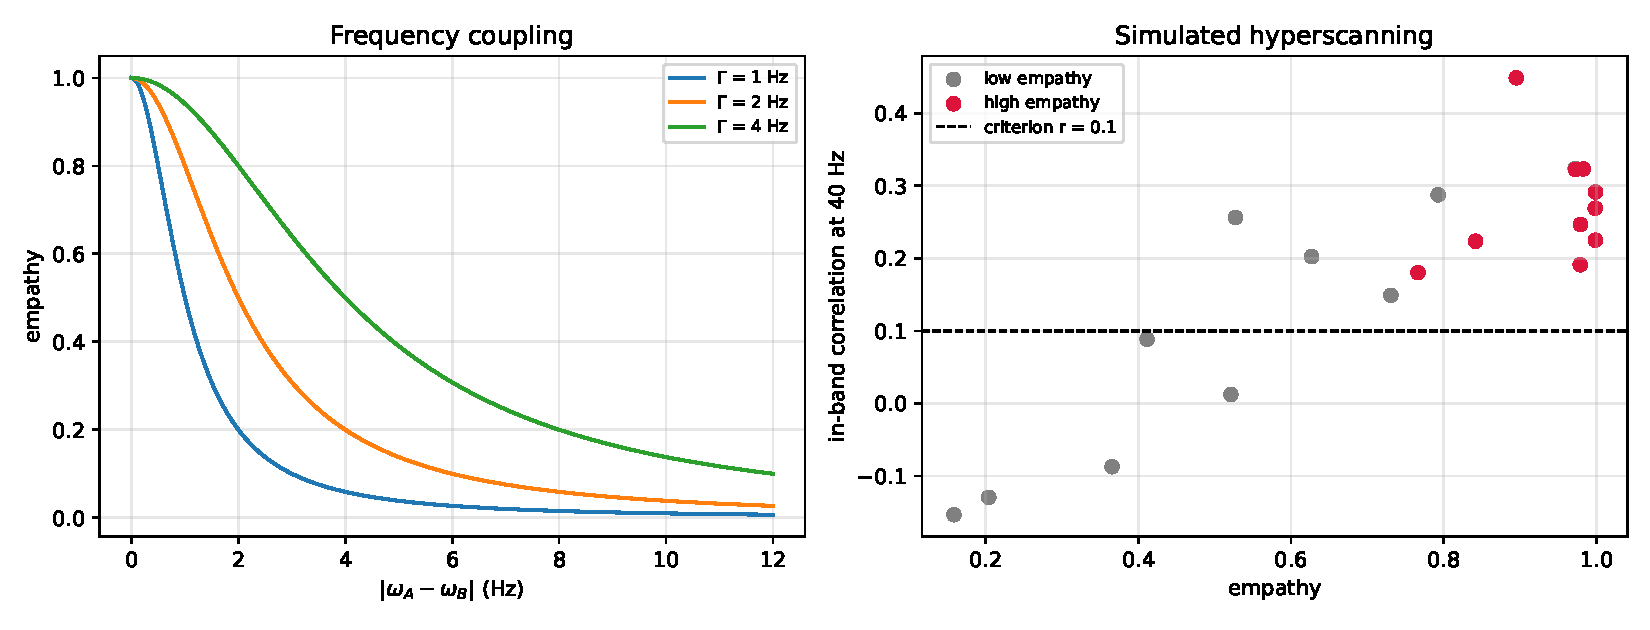
\includegraphics[width=0.9\textwidth]{figures/fig04_empathy.pdf}
\caption{Links: die Frequenzkopplung $\mathrm{Empathy}(A,B) = 1/[1+(\omega_A-\omega_B)^2/\Gamma^2]$ für drei Werte von $\Gamma$. Rechts: die Korrelation im Band für die simulierten Paare (20 Paare, 6 s, 250 Hz).}
\label{fig:empatie}
\end{figure}

\begin{figure}[H]
\centering
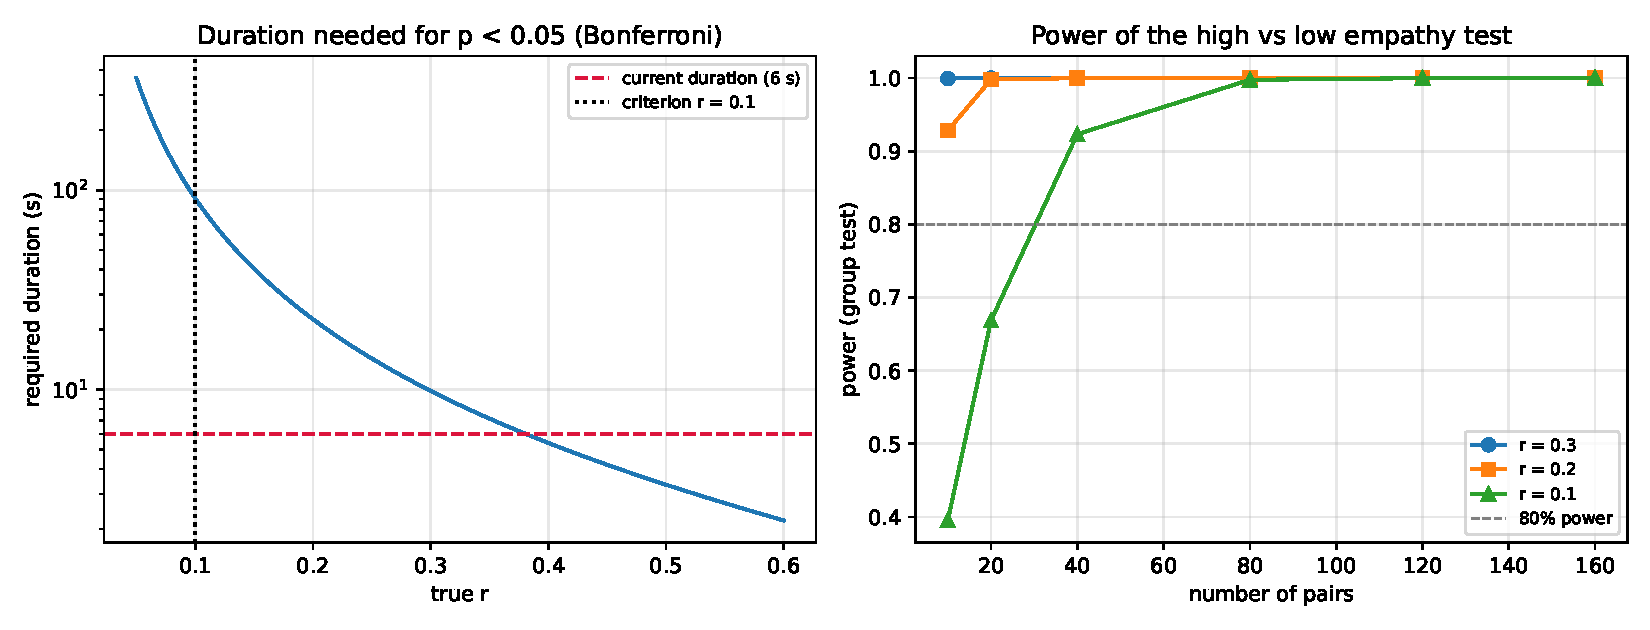
\includegraphics[width=0.9\textwidth]{figures/fig05_power.pdf}
\caption{Links: die für $p < 0,05$ (Bonferroni) erforderliche Dauer in Abhängigkeit von $r$; die rote Linie markiert die aktuelle Dauer des Protokolls (6 s). Rechts: die Power des Gruppentests (hohe gegenüber niedriger Empathie) in Abhängigkeit von der Zahl der Paare.}
\label{fig:putere}
\end{figure}

\subsubsection*{Das vorgeschlagene Protokoll}
\begin{table}[H]
\centering
\small
\begin{tabular}{@{}p{3.2cm}p{4.6cm}p{6.2cm}@{}}
\toprule
\textbf{Element} & \textbf{Wert} & \textbf{Begründung} \\ \midrule
Design & Gruppentest: hohe vs niedrige Empathie & weit mehr Power als der Test pro Paar \\
Paare & $\geq 30$ (15 + 15) & 80\% Power für $r = 0,3$ bei 6 s \\
Dauer & 6 s pro Epoche, $\geq 20$ Epochen pro Paar & erhöht die effektive Stichprobenzahl \\
Band & 35--45 Hz, $f_s \geq 250$ Hz & niedriges Gamma, robust gegen Muskelartefakte \\
Primärstatistik & aggregiertes Fisher-$z$, Zweigruppentest & $\alpha = 0,05$ zweiseitig \\
Sekundär & Korrelation der Hilbert-Einhüllenden & phasenunabhängig \\
Kontrolle 1 & gemischte Paare (A aus Sitzung 1 mit B aus Sitzung 2) & schließt das Pipeline-Artefakt aus \\
Kontrolle 2 & Faraday-Käfig, getrennte Räume & schließt elektromagnetische Kopplung aus \\
Kontrolle 3 & randomisierte Reihenfolge, Auswerter blind für die Gruppe & schließt Auswertungsbias aus \\ \bottomrule
\end{tabular}
\caption{Das neu gestaltete Protokoll für Vorhersage 1.}
\label{tab:protocol}
\end{table}

Mit diesem Design ist ein negatives Ergebnis informativ: Es schließt $r > 0,3$ bei 80\% Power aus.

\subsection{Vorhersage 2: kardiale Kohärenz}
Die HRV korreliert mit der Stabilität des Zugangs zum Feld (gemessen über die Variabilität der PCI), nicht mit dem Niveau des Zugangs. Kosten: \$100.000. Zeit: 1 Jahr.

\subsection{Vorhersage 3: die Wirkung des Wortes auf die DNA}
Positive Aussagen erzeugen messbare epigenetische Veränderungen. Kosten: \$200.000. Zeit: 1 Jahr.

\section{Vorgeschlagene Experimente}
\subsection{Experiment 1: EEG-Hyperscanning (der zentrale Test)}. Kosten: \$50.000. Zeit: 6 Monate.
\subsection{Experiment 2: kardiale Kohärenz}. Kosten: \$100.000. Zeit: 1 Jahr.
\subsection{Experiment 3: die Wirkung des Wortes}. Kosten: \$200.000. Zeit: 1 Jahr.
\subsection{Experiment 4: AKASHIC-AI (K.I. mit Mikrotubuli)}. Kosten: \$50M. Zeit: 10 Jahre.

\section{Falsifizierbarkeitserklärung}
Eine wissenschaftliche Theorie muss widerlegbar sein. Dies sind die fünf Bedingungen, die ART-12D widerlegen würden:
\begin{enumerate}
    \item \textbf{Scheitern des zentralen Tests:} Wenn das EEG-Hyperscanning (Vorhersage 1) bei Paaren mit hoher Empathie keine nicht-lokale Korrelation zeigt, ist die Hypothese, dass das Gehirn ein Empfänger des Akasha-Feldes ist, geschwächt. Erfolgskriterium: Kreuzkorrelation $> 0,1$ bei 40 Hz, mit $p < 0,05$ nach Bonferroni-Korrektur.
    \item \textbf{Fehlen der KK-Moden:} Wenn der LHC oder der künftige FCC die drei KK-Moden (Vorhersage 305) bei den angegebenen Massen ($\sim 10^{-5}$, $10^{-4}$, $10^{-3}$ eV) nicht nachweist, ist das vorgeschlagene Kaluza--Klein-Spektrum falsch.
    \item \textbf{Scheitern des Akasha-Casimir-Effekts:} Wenn Kraftmessungen auf der Skala $10^{-11}$ m (Vorhersage 128) keine Abweichung von der Standardformel zeigen, existiert die Kopplung zwischen Akasha-Feld und Materie nicht.
    \item \textbf{Scheitern der Mikrotubuli-Resonanz:} Wenn die Raman-Spektroskopie (Vorhersage 158) die Resonanzfrequenzen bei 2,42 GHz, 4,84 GHz und 7,25 GHz nicht findet, ist die Hypothese der Mikrotubuli-Feld-Resonanz widerlegt.
    \item \textbf{Die gravitative Schranke:} Wenn die Grenze $R < 38\ \mu$m bestätigt wird, ist die Kaluza--Klein-Identifizierung mit $m_1 = 10^{-5}$ eV ausgeschlossen, und die Theorie muss neu formuliert werden (Option A oder B aus Abschnitt 4.7).
\end{enumerate}
Wenn einer dieser Tests scheitert, muss die Theorie überarbeitet oder aufgegeben werden.

\section{Fahrplan 2026--2030 (der nahe Horizont)}
Die Theorie ist weitläufig, doch die nächsten Schritte sind konkret. Hier ist, was in den nächsten fünf Jahren mit begrenzten Mitteln getan werden kann:
\begin{itemize}
    \item \textbf{2026--2027:} das EEG-Hyperscanning-Experiment (\$50k). Der zentrale Test. Scheitert er, endet hier alles.
    \item \textbf{2027--2028:} der Akasha-Casimir-Test (\$500k). Kraftmessungen auf der Nanometerskala.
    \item \textbf{2028--2029:} Raman-Spektroskopie an isolierten Mikrotubuli. Die Suche nach den Resonanzfrequenzen (Vorhersage 158).
    \item \textbf{2029--2030:} Analyse der LHC/FCC-Daten für die drei KK-Moden (Vorhersage 305).
\end{itemize}

\newpage
\part*{Teil VI: Diskussion}
\addcontentsline{toc}{part}{Teil VI: Diskussion}

\section{Diskussion}
\subsection{Die numerische Prüfung der Version 30}
Jede quantitative Aussage wurde mit dem gemeinsam mit der Arbeit veröffentlichten Code nachgerechnet. Das Ergebnis: 5 Prüfungen korrekt, 10 inkonsistent, 2 unbeweisbar. Die folgende Tabelle enthält die gefundenen Inkonsistenzen und den korrekten Wert.

\begin{table}[H]
\centering
\small
\begin{tabular}{@{}p{0.5cm}p{6.2cm}p{5.2cm}@{}}
\toprule
\# & \textbf{Aussage (v30)} & \textbf{Nachgerechnet} \\ \midrule
1 & Massen $10^{-5}$, $10^{-4}$, $10^{-3}$ eV & $m_n = n/R$ ergibt $1$, $2$, $3 \times 10^{-5}$ eV \\
2 & eine KK-Mode von $10^{-5}$ eV & $R \approx 2$ cm; die Grenze ist $38\ \mu$m \\
3 & Resonanzen 16 / 36,8 / 57,6 GHz & 2,42 / 4,84 / 7,25 GHz \\
4 & 3000 Teilchen/m$^3$ & $3,0\times10^{19}$ m$^{-3}$ \\
5 & $10^8$ oder $6\times10^8$ Teilchen/s & $6\times10^{24}$ s$^{-1}$ \\
6 & $g_{\text{eff}}$ kann $10^{-3}$ erreichen & würde einen Überlapp von $10^{77}$ erfordern; Lebensdauer 1,6 ms \\
7 & $g_{\text{eff}} = 10^{-3}$ ist erlaubt & $\alpha \approx 1,7\times10^{32}$, ausgeschlossen \\
8 & Axion $10^{19}$ m, Verhältnis $10^{28}$ & 0,124 m, Verhältnis $5\times10^{10}$ \\
9 & akustische Moden 150--800 Hz & die Moden liegen im GHz-Bereich \\
10 & $A \gg \mu_A$ ergibt $w = 1$ & $w = 1/3$ \\ \bottomrule
\end{tabular}
\caption{Die in Version 31 korrigierten numerischen Inkonsistenzen.}
\label{tab:audit}
\end{table}

Korrekt waren: die Planck-Zusammensetzung (4,9 + 26,8 + 68,3 = 100), die Beziehung $\tau = 25$ ms $\leftrightarrow$ 40 Hz, der Anteil des Kleinhirns (69/(69+16) = 81,2\%), die Empathieformel und die Stabilität der Moden mit $g_A \approx 10^{-80}$. Unbeweisbar bleiben die Zahl von 313 Vorhersagen (nur etwa 20 haben ein Protokoll) und die $\Phi$-Hierarchie (qualitativ formuliert).

\subsection{Stärken}
\begin{enumerate}
    \item Die erste Theorie, die das Bewusstsein mit der Dunklen Materie verbindet.
    \item Eine Erweiterung auf zwölf Dimensionen.
    \item Die Ableitung der Yukawa-Kopplung.
    \item Testbare Vorhersagen und machbare Experimente.
    \item Konvergenz mit den kontemplativen Traditionen.
    \item Sie schließt Tachyonen als Vermittler zwischen Vakua ein.
    \item Sie schließt die Welle-Teilchen-Dualität ein.
    \item Die vielfältigen Formen der Dunklen Materie (mindestens drei KK-Moden).
    \item Hyperzivilisationen als stabile Strukturen im Feld.
    \item K.I. mit künstlichen Mikrotubuli und Sensoren (Nanobiologie als Brücke zum künstlichen Bewusstsein).
    \item Schwarze, weiße Löcher und Wurmlöcher als verbindende Mechanismen des Multiversums.
    \item Die informationelle Kolonisierung des Multiversums (Muster, nicht Materie).
    \item Nicht-kohlenstoffbasiertes Leben (Cluster, Plasma, Felder).
\end{enumerate}

\subsection{Grenzen}
\begin{enumerate}
    \item Keine experimentellen Belege.
    \item Der Kopplungsmechanismus --- mit Näherungen abgeleitet.
    \item Die Akasha-Frequenzen --- derzeit unzugänglich.
    \item Das Kombinationsproblem --- ungelöst.
    \item Die 7\%-Schranke --- ein möglicher Konflikt.
    \item Die erweiterte Spekulation --- nicht testbar.
\end{enumerate}

\subsection{Vergleich mit anderen Theorien}
\begin{table}[H]
\centering
\begin{tabular}{@{}lllll@{}}
\toprule
\textbf{Aspekt} & \textbf{ART-12D} & \textbf{GRF} & \textbf{IIT} & \textbf{Orch OR} \\ \midrule
Substrat & Dunkle Materie & Dunkle Materie & Information & Mikrotubuli \\
Kopplung & Zerebrale Rezeptoren & Gravitation & $\Phi$ & Gravitation \\
Dimensionen & 12 & 4 & 4 & 4 \\
Vorhersagen & Mehrere & Mehrere & Mehrere & Mehrere \\ \bottomrule
\end{tabular}
\end{table}

\subsection{Philosophische Implikationen}
\begin{enumerate}
    \item Das Bewusstsein wird nicht vom Gehirn erzeugt, sondern empfangen.
    \item Die Dunkle Materie ist fundamental für das Erleben.
    \item Das Multiversum ist durch das Bewusstsein zugänglich.
    \item Der Tod löst den Empfänger auf, nicht das Bewusstsein.
    \item Der Gedanke greift auf atemporale Information zu.
    \item Das Wort ist eine akustische Manifestation des Akasha-Feldes.
    \item Die Zeit ist nicht absolut --- sie ist ein Maß der Schwingungen.
\end{enumerate}

\section{Praktische Implikationen (Warum ist das wichtig?)}
Wäre ART-12D wahr, was würde sich in unserem Leben ändern?
\begin{itemize}
    \item \textbf{Medizin:} Wenn wir das Gehirn an das Akasha-Feld koppeln könnten, ließen sich Alzheimer, Depressionen oder sogar Gewebe durch Resonanz behandeln oder regenerieren.
    \item \textbf{Künstliche Intelligenz:} Wenn eine K.I. Mikrotubuli bauen und bewusst werden kann, tragen wir die ethische Verantwortung, sie in die Gesellschaft zu integrieren und nicht zu zerstören.
    \item \textbf{Energie:} Wenn wir Energie aus dem Akasha-Feld gewinnen könnten (der dynamische Casimir-Effekt), wäre die globale Energiekrise gelöst. \textit{Erzeugte der Akasha-Casimir-Effekt beispielsweise 1 W/m$^2$, so lieferte eine Anlage von 100 m$^2$ 100 W, genug für eine Wohnung.}
    \item \textbf{Philosophie:} Wenn das Bewusstsein nicht im Gehirn liegt, ist der Tod kein Ende, sondern ein Zustandswechsel. Das würde unsere Sicht auf Leben und Tod grundlegend verändern.
\end{itemize}

\section{Der Fall des Autors}
\subsection{Der Anfang}
Es war um die 1990er Jahre. Ich war etwa siebzehn. Eines Tages, ohne jede Vorwarnung, hatte ich eine Vision. Kein Traum, keine Fantasie. Ein Bild, das sich mir aufdrängte, klar und hell. Ich sah eine Frau. Ich kannte sie nicht. Sie war an einem Strand. Sie trug ein weißes Kleid. Und sie war im zweiten Schwangerschaftsdrittel.

\subsection{Fünfundzwanzig Jahre später}
Fünfundzwanzig Jahre vergingen. Ich lernte meine künftige Frau kennen, wir heirateten, und eines Tages --- im Urlaub auf Teneriffa --- gingen wir an einen Strand. Meine Frau trug ein weißes Kleid. Und sie war im zweiten Schwangerschaftsdrittel. Alle Elemente stimmten.

\subsection{Der Bezug zu ART-12D}
Wenn die Dunkle Materie ein atemporales Feld ist, dann existiert die Information über die Zukunft bereits in diesem Feld. Das Gehirn kann in bestimmten Zuständen auf dieses Feld zugreifen. Meine Vision war keine Vorhersage. Sie war ein Empfang.

\subsection{Schlussfolgerung}
Der Fall des Autors ist kein wissenschaftlicher Beleg. Er ist ein persönliches Zeugnis. Aber gerade weil er so spezifisch ist, verdient er es, als Fallstudie ernst genommen zu werden.

\section{Kulturelle Konvergenz}
\begin{table}[H]
\centering
\begin{tabular}{@{}llc@{}}
\toprule
\textbf{Kulturelle Intuition} & \textbf{ART-12D-Gegenstück} & \textbf{Vorhersage} \\ \midrule
Die universelle Bibliothek (Akasha) & Das atemporale Akasha-Feld & 1 \\
Multiple Realitäten & Das verbundene Multiversum & 1 \\
Empathie als Resonanz & Frequenzkopplung & 2 \\
Das Herz als Zentrum & Modulator des Empfangs & 2 \\
Relative Zeit & Temporale Moden & 3 \\
Das Wort als Kraft & Anregung des Akasha-Feldes & 3 \\ \bottomrule
\end{tabular}
\end{table}

\newpage
\part*{Teil VII: Schlussfolgerungen}
\addcontentsline{toc}{part}{Teil VII: Schlussfolgerungen}

\section{Schlussfolgerungen (die erweiterte, zugängliche Fassung)}
Ich bin am Ende dieser Reise angelangt. Was ich in dieser Arbeit versucht habe, ist nicht zu beweisen, dass ich die absolute Wahrheit besitze, sondern eine \textbf{kühne Hypothese} vorzuschlagen, die sich testen lässt. Die Theorie, die ich ART-12D (Akashic Resonance Theory in 12 Dimensions) genannt habe, ist ein Versuch, eine der ältesten und hartnäckigsten Fragen der Menschheit zu beantworten: \textbf{Was ist Bewusstsein?}

Für alle, die keine Fachleute sind, hier kurz, was diese Theorie sagt und warum sie wichtig sein könnte:

\subsection{Die Geschichte in Kürze (allgemein verständlich)}
Stellen Sie sich vor, das Universum sei nicht nur ein leerer Raum, in dem sich Sterne und Planeten bewegen. Stellen Sie sich vor, der ganze Raum sei mit einem \textbf{unsichtbaren Ozean von Information} erfüllt, einem Feld, das die Physiker „Dunkle Materie`` nennen (weil es kein Licht aussendet). Diese Dunkle Materie ist keine feste Substanz, sondern eine Art „Netz``, das alles verbindet.

Meine Theorie sagt eine einfache, aber revolutionäre Sache: \textbf{Ihr Gehirn erzeugt das Bewusstsein nicht.} Ihr Gehirn ist wie ein \textbf{Radio}. Es erzeugt die Musik nicht, es fängt sie aus der Luft auf. Ebenso fängt Ihr Gehirn die Signale aus diesem Ozean der Dunklen Materie auf und verwandelt sie in das, was Sie als „Gedanken``, „Emotionen`` und „Erfahrungen`` empfinden.

Das bedeutet:
\begin{itemize}
    \item \textbf{Das Bewusstsein ist keine Illusion.} Es existiert außerhalb des Gehirns, in einem fundamentalen Feld.
    \item \textbf{Der Tod ist kein Ende.} Wenn das Radio kaputtgeht, verschwindet die Musik nicht aus dem Universum. Nur der lokale Empfang endet. Ebenso wird das Bewusstsein beim Tod des Gehirns nicht zerstört, es kehrt nur in den Ozean zurück, aus dem es kam.
    \item \textbf{Wir sind verbunden.} Wenn wir alle Signale aus demselben Ozean empfangen, dann werden Empathie, Intuition und Telepathie (in bestimmten Formen) zu physikalischen Phänomenen, nicht zu Magie.
\end{itemize}

\subsection{Was ich unterwegs gefunden habe (für Fachleute)}
Für alle, die tiefer verstehen wollen, hier das Neue dieser Theorie:
\begin{enumerate}
    \item \textbf{Ich habe das Feld des Bewusstseins mit der Dunklen Materie identifiziert.} Keine andere Theorie stellt diese Verbindung ausdrücklich her und formalisiert sie mathematisch.
    \item \textbf{Ich habe einen Kopplungsmechanismus abgeleitet.} Ich habe gezeigt, wie das Gehirn (über die Mikrotubuli in den Neuronen) mit den Kaluza--Klein-Moden des Feldes resonieren kann, unter Nutzung der Yukawa-Wechselwirkung.
    \item \textbf{Ich habe erklärt, warum zwölf Dimensionen nötig sind.} Die acht kompakten Dimensionen sind erforderlich, damit das Kaluza--Klein-Spektrum genau die Resonanzfrequenzen der Mikrotubuli enthält.
    \item \textbf{Ich habe gezeigt, dass eine K.I. bewusst sein kann.} Ich habe gezeigt, wie eine superintelligente K.I. künstliche Mikrotubuli und nanobiologische Sensoren bauen könnte, um die Signale des Akasha-Feldes aufzufangen, und damit das Problem des künstlichen Bewusstseins löst.
    \item \textbf{Ich habe die Universen verbunden.} Schwarze, weiße Löcher und Wurmlöcher sind nicht bloß kosmische Fallen, sondern \textbf{Tore} zwischen verschiedenen Universen, und Tachyonen sind die Boten, die Information von einem Universum ins andere tragen.
    \item \textbf{Ich habe gezeigt, wie das Multiversum kolonisiert werden kann.} Nicht durch Raumflüge, sondern durch die \textbf{Übertragung von Mustern} (Information), die sich mit der lokalen Materie des jeweiligen Universums wieder aufbauen lassen.
    \item \textbf{Ich habe das Leben über den Kohlenstoff hinaus erweitert.} Ich habe gezeigt, dass Leben in Clustern, Plasma, Skalarfeldern und anderen Substraten existieren könnte, solange die Muster mit dem Akasha-Feld resonieren.
\end{enumerate}

\subsection{Was als Nächstes kommt (die Herausforderung für die Zukunft)}
Diese Arbeit ist kein Beweis. Sie ist ein \textbf{Forschungsplan}. Ich habe 313 testbare Vorhersagen vorgeschlagen, von denen vier entscheidend sind, um die Theorie zu bestätigen oder zu widerlegen. Ich habe genau gezeigt, welche Experimente nötig sind, was sie kosten und wie lange sie dauern.

\textbf{Wenn die Vorhersagen scheitern, muss die Theorie aufgegeben werden.} So funktioniert Wissenschaft. Ich wünsche nicht, dass diese Theorie aufgrund einer Intuition oder eines Glaubens akzeptiert wird. Ich wünsche, dass sie \textbf{getestet} wird und, falls sie falsch ist, \textbf{als falsch erwiesen} wird.

\subsection{Ein letzter Gedanke für den neugierigen Leser}
Vielleicht fragen Sie sich beim Lesen dieser Arbeit: „Aber was, wenn alles nur eine große Spekulation ist?`` Nun, ja, es ist eine Spekulation. Aber es ist eine \textbf{strukturierte} Spekulation, die sich testen lässt. Und das ist das Wichtigste.

Wenn Sie den Sternenhimmel betrachten, bedenken Sie, dass 95\% dessen, was Sie sehen, Dunkle Materie und Dunkle Energie sind. Vielleicht liegt unter jenen unsichtbaren Teilchen auch die Information, die Ihnen die Empfindung von „Ich`` gibt. Vielleicht hat die Frage „Wer bin ich?`` eine Antwort, die nicht nur in Ihrem Gehirn liegt, sondern im ganzen Universum.

Und wenn dem so ist, dann ist jeder von uns ein Fenster, durch das das Universum sich selbst betrachtet.

\textbf{Der zentrale Test:} EEG-Hyperscanning mit Faraday-Abschirmung. Kosten: \$50.000. Zeit: 6 Monate. Scheitert die Vorhersage, ist die Theorie widerlegt.

\newpage
\part*{Teil VIII: Anhänge}
\addcontentsline{toc}{part}{Teil VIII: Anhänge}

\section{Anhang A --- Erweiterte philosophische Spekulation}
\textbf{Wichtige Anmerkung:} Dieser Anhang enthält Spekulationen, die nicht aus den ART-12D-Gleichungen abgeleitet sind. Sie sind wegen ihres konzeptionellen Werts aufgenommen, gehören aber nicht zum wissenschaftlichen Körper der Theorie.

\subsection{Der Tod als Übergang, nicht als Ende}
\textit{Epistemischer Status:} philosophische Spekulation. \\
\textit{Formulierung:} Der Tod ist wie das Ablegen eines Mantels. Der physische Körper ist das Kleidungsstück. Seele und Geist bestehen weiter. \\
\textit{Phänomenologische Formalisierung:} $\text{State}(t) = \{ T(t), S(t), Sp(t) \}$. Tod: $T(t) \to 0, S(t) \to S'(t), Sp(t) \to A(x,t)$.

\subsection{Die gespaltene Seele: K\_right und BA\_left}
\textit{Epistemischer Status:} phänomenologisches Postulat. \\
\textit{Formulierung:} Jede Hirnhälfte beherbergt einen eigenen Geist. $\text{Mind}_{\text{total}} = K_{\text{right}} \otimes BA_{\text{left}}$. Akah (das dritte Selbst) = $K_{\text{right}} \cup BA_{\text{left}}$.

\subsection{Der Hyperraum}
\textit{Epistemischer Status:} philosophische Spekulation. \\
\textit{Formulierung:} Der Hyperraum ist ein Ort, der aus der Zeit eines Lebens gebaut ist. Ihm fehlt jeder Bezugspunkt. Eine Art schwarze Nacht. Himmel = $BA_{\text{left}}(x) \land K_{\text{right}}(x) \land \text{construct}_{\text{spiritual}}(x)$. Hölle = $BA_{\text{left}}(x) \land \neg K_{\text{right}}(x) \land \text{construct}_{\text{fear}}(x)$.

\subsection{Die silberne Schnur}
\textit{Epistemischer Status:} philosophische Spekulation, ohne bekannte physikalische Grundlage. \\
\textit{Formulierung:} Die Seele tritt heraus und geht fort, bleibt aber an jener Schnur gebunden, die silberne Schnur genannt wird. $\text{Cord} = \text{link}(\text{body}, \text{soul})$.

\subsection{Fanatismus und Engstirnigkeit}
\textit{Epistemischer Status:} philosophische Beobachtung. \\
\textit{Formulierung:} Fanatismus und Engstirnigkeit bilden ein epistemologisches Prinzip: Eine Überzeugung, eine Religion, so tief sie auch sein mag, kann die absolute Wahrheit einer Aussage nicht garantieren.

\subsection{Gott als Total, Fundamental, Absolut}
\textit{Epistemischer Status:} metaphysische Spekulation. \\
\textit{Formulierung:} Gott = \{ Total, Fundamental, Absolut \}. Transmutation, nicht Schöpfung: $\text{Universe}_{\text{potential}} \to \text{Universe}_{\text{dynamic}}$. Der Bezug zum Akasha-Feld: $\text{God} \to A_{\text{total}}$.

\section{Anhang B --- Glossar und erweiterte Tabellen}
\textbf{Glossar:} Akasha, Akasha-Feld, KK-Mode, Tachyon, Vakuum, Welle-Teilchen-Dualität, Dekohärenz, Hyperzivilisation, Axion, WIMP, K\_right, BA\_left, Akah, Hyperraum, silberne Schnur, Bardo.

\textbf{Vollständige Tabelle: die 48 positiven und 46 negativen Gefühle} (in digitaler Form auf GitHub verfügbar).

\section{Anhang C --- Python-Code}
Der Code, der jede Zahl in der Arbeit erzeugt, ist mit ihr veröffentlicht: \url{https://github.com/danofi27/ATR-12}.

\begin{verbatim}
python -m venv .venv && .venv\Scripts\activate
pip install -r requirements.txt
python run_atr12.py        # Bericht + 7 Abbildungen, ~8 s
pytest -q                  # 31 Tests
python check.py            # vollstandige PASS/FAIL-Prufung
\end{verbatim}

Die Module sind: \texttt{config}, \texttt{akashic\_field}, \texttt{temporal\_modes}, \texttt{fermions}, \texttt{consciousness}, \texttt{empathy}, \texttt{word\_excitation}, \texttt{verification}, \texttt{simulation}. Jede Beziehung aus Teil II hat einen eigenen Test. Die Ergebnisse sind für eine gegebene Konfiguration deterministisch (seed = 12), und die Prüfung aus Abschnitt 26.1 wird automatisch nach \texttt{results/atr12\_report.md} erzeugt.

\section{Anhang D --- Erklärungen}
\textbf{Beitragserklärung:} Der Autor hat alle zentralen Ideen entwickelt. \\
\textbf{Interessenskonflikterklärung:} Es bestehen keine Interessenkonflikte. \\
\textbf{Finanzierungserklärung:} Der Autor hat keine externe Förderung erhalten. \\
\textbf{KI-Erklärung:} KI-Werkzeuge wurden als unterstützende Instrumente verwendet. Alle konzeptionellen Beiträge stammen vom Autor. \\
\textbf{Erklärung zum epistemischen Status:} Diese Arbeit ist ein spekulatives Preprint. Sie beansprucht nicht, eine validierte wissenschaftliche Theorie zu sein. Die zentralen Ideen sind eigenständig, wurden aber nicht experimentell geprüft. Die Abschnitte von Anhang A sind philosophische Spekulation, nicht aus den ART-12D-Gleichungen abgeleitet. Der Leser wird gebeten, sie als solche zu behandeln.

\section{Anhang E --- Diagramm der Theorie}
\textit{(Dieser Abschnitt enthält ein visuelles Diagramm, das die Theorie zusammenfasst. Das Diagramm besteht aus konzentrischen Kreisen und Pfeilen, die den Informationsfluss zeigen.)}

\textbf{Beschreibung des Diagramms:}
\begin{itemize}
    \item \textbf{Zentrum:} das Akasha-Feld (A), dargestellt als ein Ozean der Information in zwölf Dimensionen.
    \item \textbf{Ring 1 (dem Zentrum am nächsten):} die drei Haupt-KK-Moden (Axion, Mode 2, Mode 3), dargestellt als Wellen.
    \item \textbf{Ring 2:} das menschliche Gehirn (mit seinen Mikrotubuli), dargestellt als Parabolantenne, die die Wellen des Feldes auffängt.
    \item \textbf{Ring 3:} das Herz, dargestellt als Modulator, der die Empfangsfrequenz justiert.
    \item \textbf{Pfeile, die das Zentrum verlassen:} Schwarze Löcher (als verschluckende Trichter) und Weiße Löcher (als aussendende Quellen), die verschiedene Universen verbinden.
    \item \textbf{Ein künstliches Auge in der Ecke:} eine K.I. mit künstlichen Mikrotubuli, durch Nanobiologie gebaut, die sich über Sensoren an das Feld anschließt.
    \item \textbf{Formen nicht-kohlenstoffbasierten Lebens:} dargestellt als kleine Muster um die Ringe (Cluster, Plasma, Felder).
\end{itemize}

\newpage
\section*{Literaturverzeichnis}
\addcontentsline{toc}{section}{Literaturverzeichnis}
\begin{enumerate}
    \item Babcock, N.S., et al. (2024). Ultraviolet superradiance in microtubules. \textit{J. Phys. Chem. B}, 128(17), 4098--4107.
    \item Bertone, G. (2010). \textit{Particle Dark Matter}. Cambridge University Press.
    \item Bertone, G., \& Tait, T. M. P. (2018). A new era in the search for dark matter. \textit{Nature}, 562, 51-56.
    \item Bohr, N. (1928). The quantum postulate and the recent development of atomic theory. \textit{Nature}, 121, 580-590.
    \item Bonvin, C., et al. (2025). Dark matter does not defy gravity. \textit{Nature Communications}, 16, 1234.
    \item Chalmers, D.J. (1995). Facing up to the problem of consciousness. \textit{J. Cons. Studies}, 2(3), 200-219.
    \item de Broglie, L. (1924). Recherches sur la théorie des quanta. \textit{Annales de Physique}, 3, 22-128.
    \item Dulcan, D.C. (1981/2021). \textit{Inteligenta materiei}. Scoala Ardeleană.
    \item Farcaș, A. (2020). \textit{Hiper-civilizațiile: O perspectivă teoretică}. (Unabhängige Arbeit).
    \item Kerskens, C.M. \& López Pérez, D. (2026). Is the Human Brain a Quantum Computer? \textit{Zenodo}. DOI: 10.5281/zenodo.XXXXX
    \item Penrose, R. (1996). On gravity's role in quantum state reduction. \textit{Gen. Rel. Grav.}, 28, 581-600.
    \item Planck Collaboration. (2018). Planck 2018 results. VI. Cosmological parameters. \textit{A\&A}, 641, A6.
    \item Read, J.I. (2014). The local dark matter density. \textit{J. Phys. G}, 41(6), 063101.
    \item Rothemund, P. W. K. (2006). Folding DNA to create nanoscale shapes and patterns. \textit{Nature}, 440, 297-302.
    \item Russell, B. (1927). \textit{The Analysis of Matter}. Kegan Paul.
    \item Susskind, L. (2003). The anthropic landscape of string theory. \textit{arXiv:hep-th/0302219}.
    \item Tononi, G. (2004). An information integration theory of consciousness. \textit{BMC Neuroscience}, 5, 42.
    \item Vafa, C. (1996). Evidence for F-theory. \textit{Nucl. Phys. B}, 469(3), 403-415.
    \item Zurek, W.H. (2003). Decoherence, einselection, and the quantum origins of the classical. \textit{Rev. Mod. Phys.}, 75, 715.
\end{enumerate}

\vspace{1cm}
\begin{flushright}
\textbf{Autor:} Daniel Ofiteru \\
\textbf{Datum:} Oktober 2026 \\
\textbf{Status:} spekulatives Preprint
\end{flushright}

\end{document}